\documentclass{article}
\usepackage{fancyhdr}
\usepackage{ctex}
\usepackage{listings}
\usepackage{graphicx}
\usepackage[a4paper, body={18cm,22cm}]{geometry}
\usepackage{amsmath,amssymb,amstext,wasysym,enumerate,graphicx}
\usepackage{float,abstract,booktabs,indentfirst,amsmath}
\usepackage{array}
\usepackage{booktabs}
\usepackage{multirow}
\usepackage{url}
\usepackage{diagbox}
\usepackage{hyperref}
\usepackage{listings}
\renewcommand\arraystretch{1.4}
\usepackage{indentfirst}
\setlength{\parindent}{2em}
\usepackage{enumitem}
\usepackage{accsupp}
\setmonofont{Consolas}
\usepackage{listings}
\usepackage{xcolor}
\usepackage{makecell}
\usepackage{subfigure}
\usepackage{longtable}
\usepackage{forest}
\setCJKmonofont{黑体}
\newcommand\emptyaccsupp[1]{\BeginAccSupp{ActualText={}}#1\EndAccSupp{}}
\newcommand\SQL{\texttt{SQL}}
\renewcommand\tt{\texttt}
\lstset{
    % language = C,
    showstringspaces=false,
    xleftmargin = 3em,xrightmargin = 3em, aboveskip = 1em,
	backgroundcolor = \color{white}, % 背景色
	basicstyle = \small\ttfamily, % 基本样式 + 小号字体
	rulesepcolor= \color{gray}, % 代码块边框颜色
	breaklines = true, % 代码过长则换行
	numbers = left, % 行号在左侧显示
	numberstyle=\emptyaccsupp,
    numbersep = 14pt, 
    keywordstyle=\color{purple}\bfseries, % 关键字颜色
    commentstyle =\color{red!50!green!50!blue!60}, % 注释颜色
    stringstyle = \color{red}, % 字符串颜色
    morekeywords={ASSERT, int64_t, uint32_t},
	% frame = shadowbox, % 用(带影子效果)方框框住代码块
	frame = single, % 用(带影子效果)方框框住代码块
	showspaces = false, % 不显示空格
	columns = fixed, % 字间距固定
  framesep=1em,
  tabsize=2,
} 
\lstset{
    sensitive=true,
    moreemph={ASSERT, NULL}, emphstyle=\color{red}\bfseries,
    moreemph=[2]{int64_t, uint32_t, tid_t, uint8_t, int16_t, uint16_t, int32_t, size_t}, emphstyle=[2]\color{purple}\bfseries,
    showspaces = false, % 不显示空格
    }
%--------------------页眉--------------------%
\pagestyle{fancy}
\fancyhead[L]{}
\fancyhead[R]{}
\fancyhead[C]{《数据库系统及应用实践》课程实验报告}
\fancyfoot[C]{-\thepage-}
\renewcommand{\headrulewidth}{1.5pt}
%--------------------标题--------------------%
\begin{document}
\begin{center}
  \LARGE{{\textbf{\heiti 《数据库系统及应用实践》课程实验报告}}}

  \vspace{0.5em}

  \large 实验6:查询处理
  \begin{table}[H]
    \centering
    \begin{tabular}{p{2cm}p{2cm}<{\centering}p{0.4cm}p{2cm}p{3cm}<{\centering}p{0.4cm}p{2cm}p{3cm}<{\centering}}
      姓\qquad 名: & 李鹏达 & \quad & 学\qquad 号: & 10225101460 & \quad & 完成日期: & 2024年6月11日 \\ \cline{2-2} \cline{5-5} \cline{8-8}
    \end{tabular}
  \end{table}
\end{center}
% \rule{\textwidth}{1pt}
%--------------------正文--------------------%
\section{实验目标}
  学习MySQL数据库管理系统中显示查询执行计划的基本方法,理解查询处理的基本流程,并能够根据执行计划对查询性能进行分析和优化。

\section{实验过程记录}

\subsection{TPC-H基准测试查询分析}

\begin{itemize}
  \item 使用 EXPLAIN 分析实验5中的22个TPC-H查询;
  \begin{itemize}[label=\(\circ\)]
    \item 记录所生成的查询计划
    \item 对比估计代价和实际执行时间的差别
    \item 分析是否能够通过创建索引、更新统计数据等手段来优化查询的性能
  \end{itemize}
  \item 根据分析的结果对系统进行优化
  \begin{itemize}[label=\(\circ\)]
    \item 记录优化后所生成的查询计划
    \item 对比优化前后的执行计划,说明优化手段是否有效
  \end{itemize}
\end{itemize}

\subsubsection{分析}

\begin{enumerate}
  \item Q1

\begin{lstlisting}[language=sql]
select l_returnflag, l_linestatus, sum(l_quantity) as sum_qty,
sum(l_extendedprice) as sum_base_price, sum(l_extendedprice*(1-l_discount)) as
sum_disc_price, sum(l_extendedprice*(1-l_discount)*(1+l_tax)) as sum_charge,
avg(l_quantity) as avg_qty, avg(l_extendedprice) as avg_price,
avg(l_discount) as avg_disc, count(*) as count_order from lineitem where
l_shipdate <= date '1998-12-01' - interval '90' day group by l_returnflag,
l_linestatus order by l_returnflag, l_linestatus;
\end{lstlisting}

\begin{figure}[H]
\centering
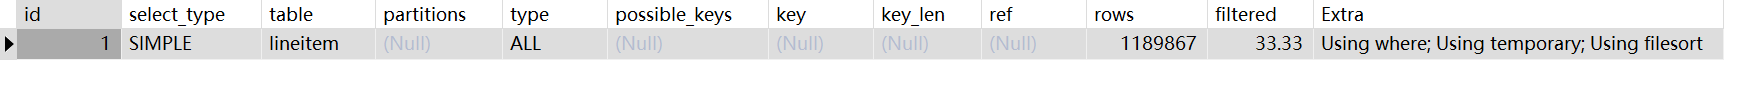
\includegraphics[width=0.9\textwidth]{img/1.png}
\caption{Q1查询 \tt{EXPLAIN} 结果}
\end{figure}

\begin{figure}[H]
\centering
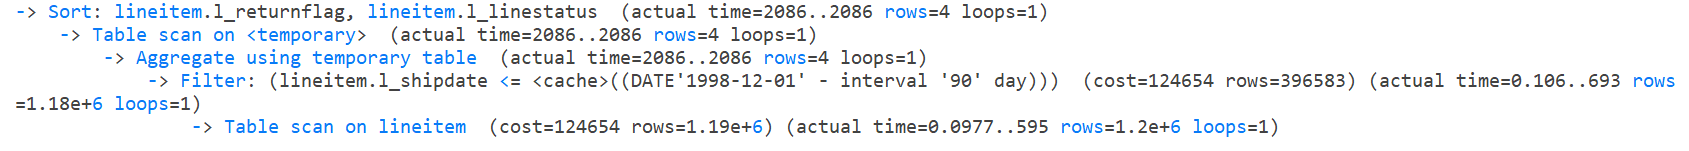
\includegraphics[width=0.9\textwidth]{img/2.png}
\caption{Q1查询 \tt{EXPLAIN ANALYZE} 结果}
\end{figure}

\begin{figure}[H]
  \centering
  \begin{forest}
  for tree={
    grow=south,
    draw,
    rounded corners,
    edge={->},
    node options={align=center}
  }
  [Sort: \tt{l\_returnflag, l\_linestatus}
    [Table scan on \tt{<temporary>}
      [Aggregate using temporary table
        [Filter: \tt{l\_shipdate <= (DATE'1998-12-01' - interval '90' day)}
          [Table scan on \tt{lineitem}]
        ]
      ]
    ]
  ]
  \end{forest}
  \caption{Q1查询执行计划}
\end{figure}

可以看到,Q1查询的执行计划中使用了临时表,对 \tt{lineitem} 表进行了全表扫描,没有使用索引,导致查询性能较差。可以通过为 \tt{lineitem} 表的 \tt{l\_shipdate} 字段创建索引来优化查询性能。

\item Q2

\begin{lstlisting}[language=sql]
select s_acctbal, s_name, n_name, p_partkey, p_mfgr, s_address, s_phone,
s_comment from part, supplier, partsupp, nation, region where p_partkey
= ps_partkey and s_suppkey = ps_suppkey and p_size = 15 and p_type like
'%BRASS' and s_nationkey = n_nationkey and n_regionkey = r_regionkey and
r_name = 'EUROPE' and ps_supplycost = ( select min(ps_supplycost) from
partsupp, supplier, nation, region where p_partkey = ps_partkey and
s_suppkey = ps_suppkey and s_nationkey = n_nationkey and n_regionkey =
r_regionkey and r_name = 'EUROPE' ) order by s_acctbal desc, n_name,
s_name, p_partkey;
\end{lstlisting}

\begin{figure}[H]
\centering
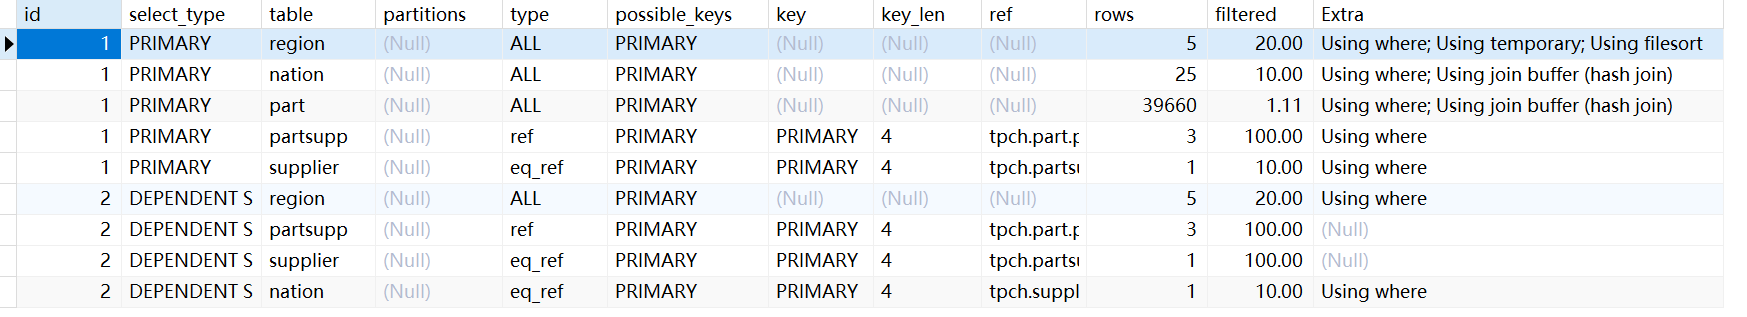
\includegraphics[width=0.9\textwidth]{img/3.png}
\caption{Q2查询 \tt{EXPLAIN} 结果}
\end{figure}

\begin{figure}[H]
\centering
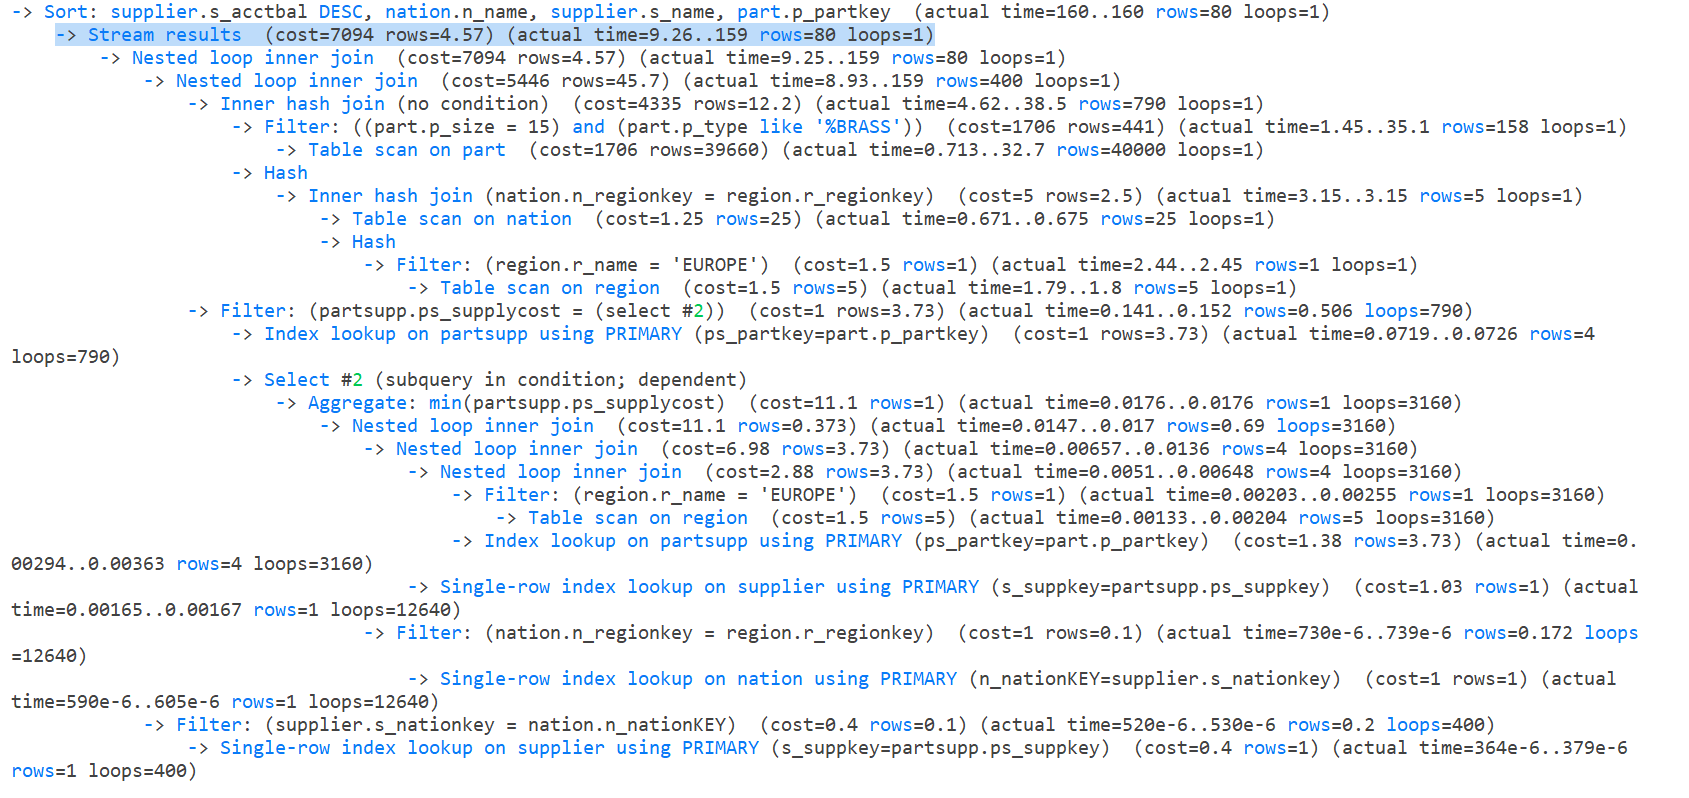
\includegraphics[width=0.9\textwidth]{img/4.png}
\caption{Q2查询 \tt{EXPLAIN ANALYZE} 结果}
\end{figure}

\begin{figure}[H]
  \centering
    \resizebox{0.8\textwidth}{!}{
      \begin{forest}
      for tree={
        grow=south,
        draw,
        rounded corners,
        edge={->},
        node options={align=center, text width=10em}
      }
      [Sort: \tt{supplier.s\_acctbal DESC, nation.n\_name, supplier.s\_name, part.p\_partkey}
        [Stream results
          [Nested loop inner join
            [Nested loop inner join
              [Inner hash join (no condition)
                [Filter: \tt{part.p\_size = 15} and \tt{part.p\_type like '\%BRASS'}
                  [Table scan on \tt{part}]
                ]
                [Hash
                  [Inner hash join (nation.n\_regionkey = region.r\_regionkey)
                    [Table scan on \tt{nation}]
                    [Hash
                      [Filter: \tt{region.r\_name = 'EUROPE'}
                        [Table scan on \tt{region}]
                      ]
                    ]
                  ]
                ]
              ]
              [Filter: \tt{partsupp.ps\_supplycost = (select \#2)}
                [Index lookup on \tt{partsupp} using PRIMARY \tt{(ps\_partkey=part.p\_partkey)}]
                [Select \#2 (subquery in condition; dependent)
                  [Aggregate: \tt{min(partsupp.ps\_supplycost)}
                    [Nested loop inner join
                      [Nested loop inner join
                        [Nested loop inner join
                          [Filter: \tt{region.r\_name = 'EUROPE'}
                            [Table scan on \tt{region}]
                          ]
                          [Index lookup on \tt{partsupp} using PRIMARY \tt{(ps\_partkey=part.p\_partkey)}]
                        ]
                        [Single-row index lookup on \tt{supplier} using PRIMARY \tt{(s\_suppkey=partsupp.ps\_suppkey)}]
                      ]
                      [Filter: \tt{nation.n\_regionkey = region.r\_regionkey}
                        [Single-row index lookup on \tt{nation} using PRIMARY \tt{(n\_nationKEY=supplier.s\_nationkey)}]
                      ]
                    ]
                  ]
                ]
              ]
            ]
            [Filter: \tt{supplier.s\_nationkey = nation.n\_nationKEY}
              [Single-row index lookup on \tt{supplier} using PRIMARY (s\_suppkey=partsupp.ps\_suppkey)]
            ]
          ]
        ]
      ]
      \end{forest}
    }
  \caption{Q2查询执行计划}
\end{figure}

可以看到,Q2查询的执行计划中,对\tt{region},\tt{nation}和\tt{part} 表进行了全表扫描,没有使用索引,导致查询性能较差。可以通过为 \tt{region},\tt{nation}和\tt{part} 表的相关字段创建索引来优化查询性能。

\item Q3

\begin{lstlisting}[language=sql]
select 
  l_orderkey, sum(l_extendedprice*(1-l_discount)) as revenue,
  o_orderdate, o_shippriority 
from customer, orders, lineitem 
where
  c_mktsegment = 'BUILDING' and c_custkey = o_custkey 
  and l_orderkey = o_orderkey and o_orderdate < date '1995-03-15' 
  and l_shipdate > date '1995-03-15' 
group by l_orderkey, o_orderdate, o_shippriority 
order by revenue desc, o_orderdate;
\end{lstlisting}

\begin{figure}[H]
\centering
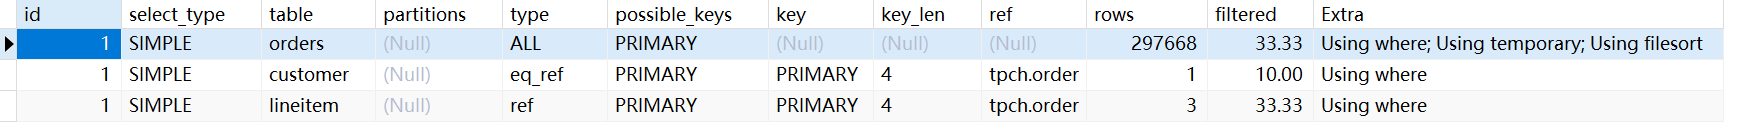
\includegraphics[width=1\textwidth]{img/5.png}
\caption{Q3查询 \tt{EXPLAIN} 结果}
\end{figure}

\begin{figure}[H]
\centering
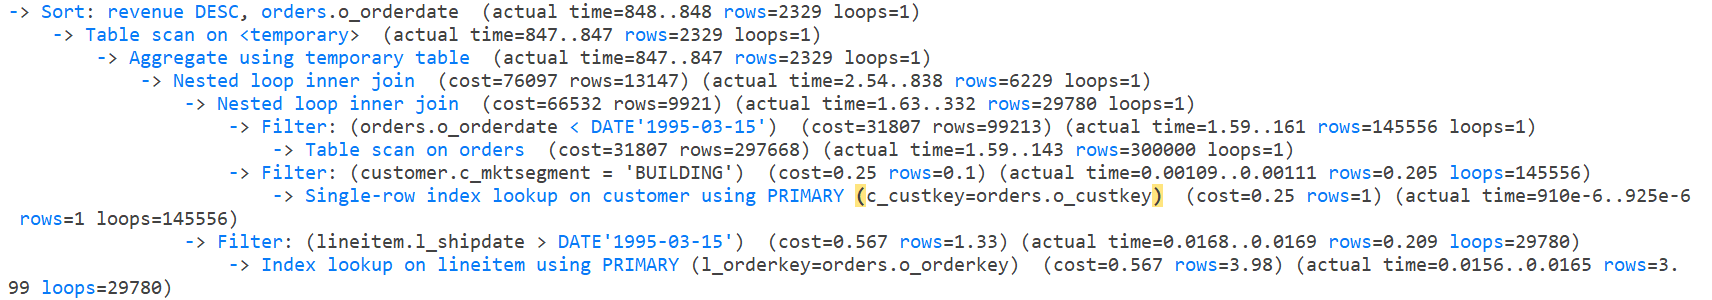
\includegraphics[width=1\textwidth]{img/6.png}
\caption{Q3查询 \tt{EXPLAIN ANALYZE} 结果}
\end{figure}

\begin{figure}[H]
  \centering
  \resizebox{\textwidth}{!}{
    \begin{forest}
    for tree={
      grow=south,
      draw,
      rounded corners,
      edge={->},
      node options={align=center, text width=15em}
    }
    [Sort: \tt{revenue DESC, orders.o\_orderdate}
        [Table scan on \tt{<temporary>}
            [Aggregate using temporary table
                [Nested loop inner join
                    [Nested loop inner join
                        [Filter: (\tt{orders.o\_orderdate} < \tt{DATE'1995-03-15'})
                            [Table scan on \tt{orders}]
                        ]
                        [Filter: (\tt{customer.c\_mktsegment} \tt{=} 'BUILDING')
                            [Single-row index lookup on \tt{customer} using PRIMARY (\tt{c\_custkey\tt{=}orders.o\_custkey})]
                        ]
                    ]
                    [Filter: (\tt{lineitem.l\_shipdate} > \tt{DATE'1995-03-15'})
                        [Index lookup on \tt{lineitem} using PRIMARY (\tt{l\_orderkey\tt{=}orders.o\_orderkey})]
                    ]
                ]
            ]
        ]
    ]
    \end{forest}
  }
  \caption{Q3查询执行计划}
\end{figure}

可以看到,Q3查询的执行计划中,对\tt{orders}表进行了全表扫描,没有使用索引,导致查询性能较差。可以通过为 \tt{orders} 的 \tt{o\_orderdate} 字段创建索引来优化查询性能。

\item Q4

\begin{lstlisting}[language=sql]
select o_orderpriority, count(*) as order_count 
from orders 
where
  o_orderdate >= date '1993-07-01' 
  and o_orderdate < date '1993-07-01' + interval '3' month 
  and exists ( 
    select * from lineitem 
    where l_orderkey = o_orderkey and l_commitdate < l_receiptdate 
  ) 
group by o_orderpriority 
order by o_orderpriority;
\end{lstlisting}

\begin{figure}[H]
\centering
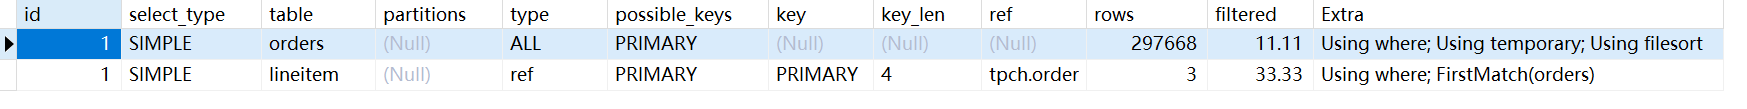
\includegraphics[width=1\textwidth]{img/7.png}
\caption{Q4查询 \tt{EXPLAIN} 结果}
\end{figure}

\begin{figure}[H]
\centering
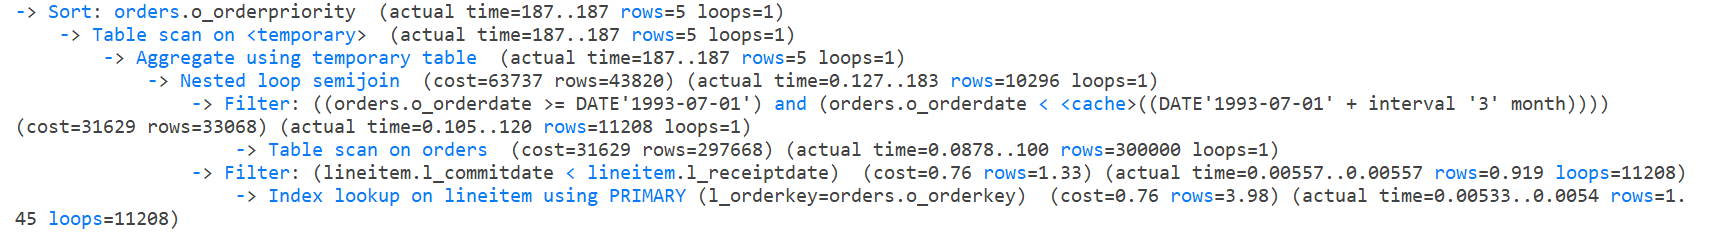
\includegraphics[width=1\textwidth]{img/8.png}
\caption{Q4查询 \tt{EXPLAIN ANALYZE} 结果}
\end{figure}


\begin{figure}[H]
  \centering
  \resizebox{0.6\textwidth}{!}{
    \begin{forest}
    for tree={
      grow=south,
      draw,
      rounded corners,
      edge={->},
      node options={align=center, text width=15em}
    }
    [Sort: \tt{orders.o\_orderpriority}
        [Table scan on \tt{<temporary>}
            [Aggregate using temporary table
                [Nested loop semijoin
                    [Filter: ((\tt{orders.o\_orderdate >= }\tt{DATE'1993-07-01'}) and (\tt{orders.o\_orderdate} < <cache>((\tt{DATE'1993-07-01'} + interval '3' month)))) 
                        [Table scan on \tt{orders}]
                    ]
                    [Filter: (\tt{lineitem.l\_commitdate} < \tt{lineitem.l\_receiptdate})
                        [Index lookup on \tt{lineitem} using PRIMARY (\tt{l\_orderkey=orders.o\_orderkey})]
                    ]
                ]
            ]
        ]
    ]
    \end{forest}
  }
  \caption{Q4查询执行计划}
\end{figure}

可以看到,Q4查询的执行计划中,对\tt{orders}表进行了全表扫描,没有使用索引,导致查询性能较差。可以通过为 \tt{orders} 的 \tt{o\_orderdate} 字段创建索引来优化查询性能。

\item Q5

\begin{lstlisting}[language=sql]
select n_name, sum(l_extendedprice * (1 - l_discount)) as revenue 
from customer, orders, lineitem, supplier, nation, region 
where 
  c_custkey = o_custkey and l_orderkey = o_orderkey and l_suppkey = s_suppkey 
  and c_nationkey = s_nationkey and s_nationkey = n_nationkey 
  and n_regionkey = r_regionkey and r_name = 'ASIA' and o_orderdate >= date '1994-01-01' 
  and o_orderdate < date '1994-01-01' + interval '1' year 
group by n_name 
order by revenue desc;
\end{lstlisting}

\begin{figure}[H]
\centering
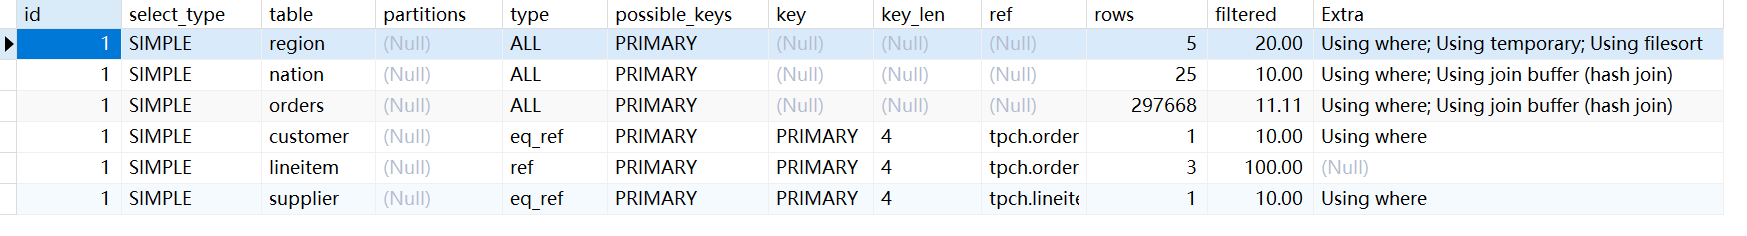
\includegraphics[width=0.85\textwidth]{img/9.png}
\caption{Q5查询 \tt{EXPLAIN} 结果}

\end{figure}

\begin{figure}[H]
\centering
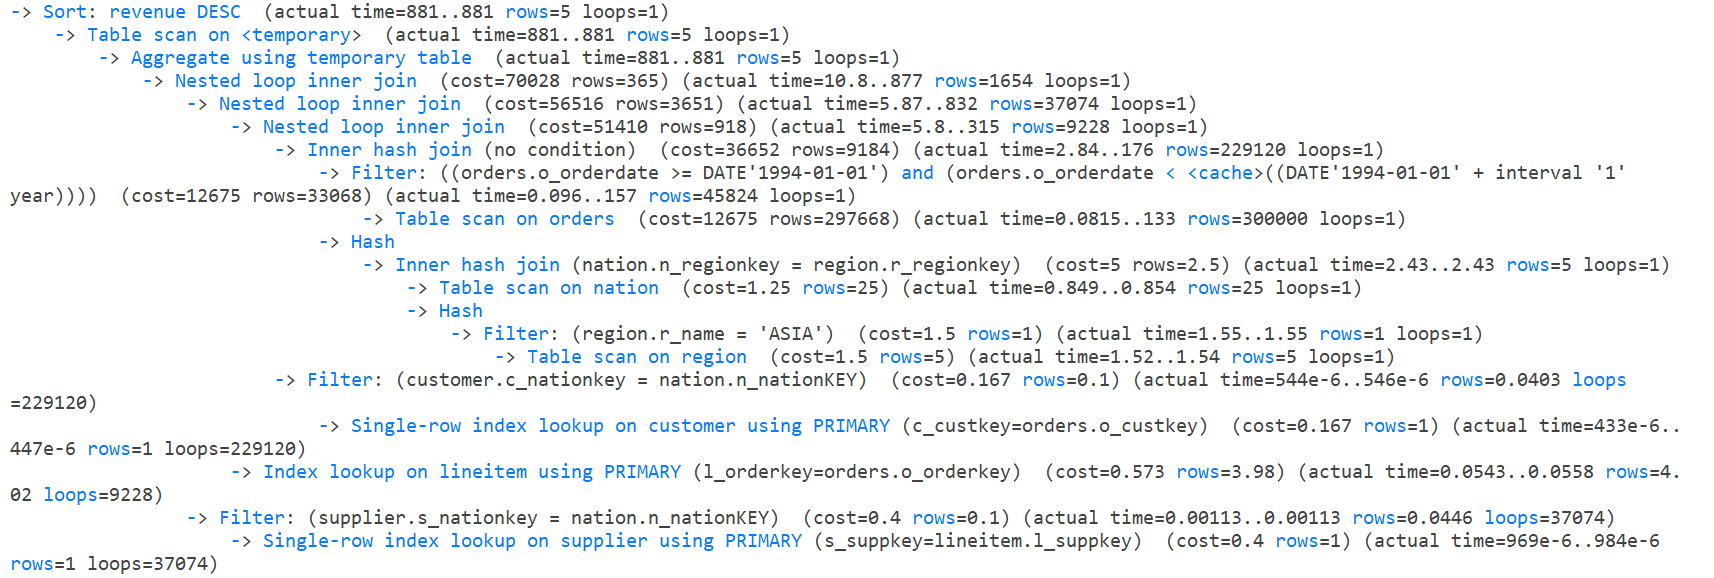
\includegraphics[width=0.85\textwidth]{img/10.png}
\caption{Q5查询 \tt{EXPLAIN ANALYZE} 结果}
\end{figure}

\begin{figure}[H]
  \centering
  \resizebox{0.85\textwidth}{!}{
    \begin{forest}
    for tree={
      grow=south,
      draw,
      rounded corners,
      edge={->},
      node options={align=center, text width=15em}
    }
    [Sort: \tt{revenue DESC}
        [Table scan on \tt{<temporary>}
            [Aggregate using temporary table
                [Nested loop inner join
                    [Nested loop inner join
                        [Nested loop inner join
                            [Inner hash join (no condition)
                                [Filter: ((\tt{orders.o\_orderdate} \tt{>=} \tt{DATE'1994-01-01'}) \tt{and} (\tt{orders.o\_orderdate} \tt{<} \tt{<cache>}((\tt{DATE'1994-01-01'} + interval '1' year))))
                                    [Table scan on \tt{orders}]
                                ]
                                [Hash
                                    [Inner hash join (\tt{nation.n\_regionkey} \tt{=} \tt{region.r\_regionkey})
                                        [Table scan on \tt{nation}]
                                        [Hash
                                            [Filter: (\tt{region.r\_name} \tt{=} 'ASIA')
                                                [Table scan on \tt{region}]
                                            ]
                                        ]
                                    ]
                                ]
                            ]
                            [Filter: (\tt{customer.c\_nationkey} \tt{=} \tt{nation.n\_nationKEY})
                                [Single-row index lookup on \tt{customer} using PRIMARY (\tt{c\_custkey=orders.o\_custkey})]
                            ]
                        ]
                        [Index lookup on \tt{lineitem} using PRIMARY (\tt{l\_orderkey=orders.o\_orderkey})]
                    ]
                    [Filter: (\tt{supplier.s\_nationkey} \tt{=} \tt{nation.n\_nationKEY})
                        [Single-row index lookup on \tt{supplier} using PRIMARY (\tt{s\_suppkey=lineitem.l\_suppkey})]
                    ]
                ]
            ]
        ]
    ]
    \end{forest}
  }
  \caption{Q5查询执行计划}
\end{figure}

可以看到,Q5查询的执行计划中,对\tt{region},\tt{nation}和\tt{orders} 表进行了全表扫描,没有使用索引,导致查询性能较差。可以通过为 \tt{region},\tt{nation}和\tt{orders} 表的相关字段创建索引来优化查询性能。

通过比较 \tt{cost} 可以发现,在扫描 \tt{orders} 表时,\tt{cost} 较高,因此应优先优化 \tt{orders} 表的查询性能。

\item Q6

\begin{lstlisting}[language=sql]
select sum(l_extendedprice*l_discount) as revenue 
from lineitem 
where 
  l_shipdate >= date '1994-01-01' 
  and l_shipdate < date '1994-01-01' + interval '1' year 
  and l_discount between 0.06 - 0.01 and 0.06 + 0.01 
  and l_quantity < 24;
\end{lstlisting}

\begin{figure}[H]
\centering
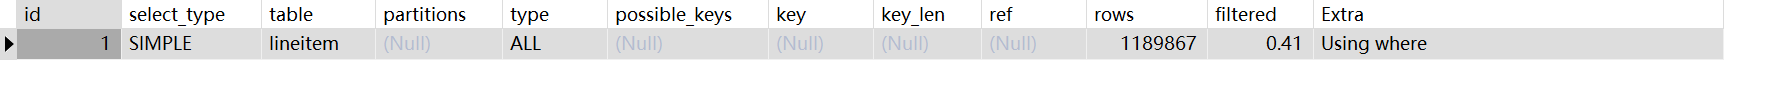
\includegraphics[width=\textwidth]{img/11.png}
\caption{Q6查询 \tt{EXPLAIN} 结果}
\end{figure}

\begin{figure}[H]
\centering
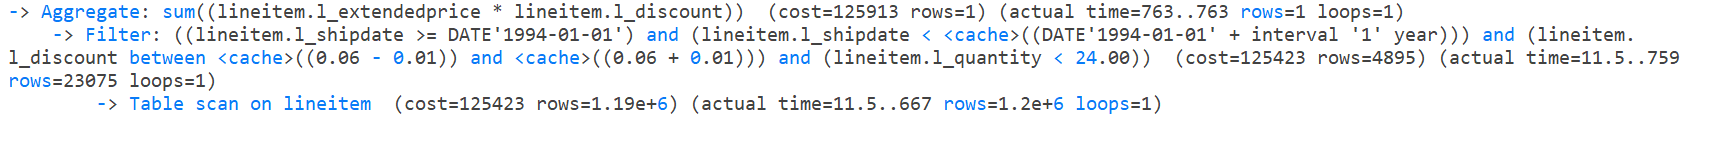
\includegraphics[width=\textwidth]{img/12.png}
\caption{Q6查询 \tt{EXPLAIN ANALYZE} 结果}
\end{figure}

\begin{figure}[H]
  \centering
  % \resizebox{0.6\textwidth}{!}{
    \begin{forest}
    for tree={
      grow=south,
      draw,
      rounded corners,
      edge={->},
      node options={align=center, text width=15em}
    }
    [Aggregate: \tt{sum((lineitem.l\_extendedprice * lineitem.l\_discount))}
        [Filter
          [Table scan on \tt{lineitem}]
        ]
    ]
    \end{forest}
  % }
  \caption{Q6查询执行计划}
\end{figure}

可以看到,Q6查询的执行计划中,对\tt{lineitem}表进行了全表扫描,没有使用索引,导致查询性能较差。可以通过为 \tt{lineitem} 表的 \tt{l\_shipdate},\tt{l\_discount} 和 \tt{l\_quantity} 字段创建索引来优化查询性能。

通过比较 \tt{rows} 字段可以发现,在进行\tt{Filter}时,预期的行数要远远小于实际的行数。

\item Q7

\begin{lstlisting}[language=sql]
select supp_nation, cust_nation, l_year, sum(volume) as revenue 
from ( 
  select n1.n_name as supp_nation, n2.n_name as cust_nation, 
    extract( year from l_shipdate) as l_year, 
    l_extendedprice * (1 - l_discount) as volume 
  from supplier, lineitem, orders, customer, nation n1, nation n2 
  where
    s_suppkey = l_suppkey and o_orderkey = l_orderkey 
    and c_custkey = o_custkey and s_nationkey = n1.n_nationkey 
    and c_nationkey = n2.n_nationkey 
    and (
      (n1.n_name = 'FRANCE' and n2.n_name = 'GERMANY') 
      or (n1.n_name = 'GERMANY' and n2.n_name = 'FRANCE') 
    ) 
    and l_shipdate between date '1995-01-01' and date '1996-12-31' 
) as shipping 
group by supp_nation, cust_nation, l_year 
order by supp_nation, cust_nation, l_year;
\end{lstlisting}

\begin{figure}[H]
\centering
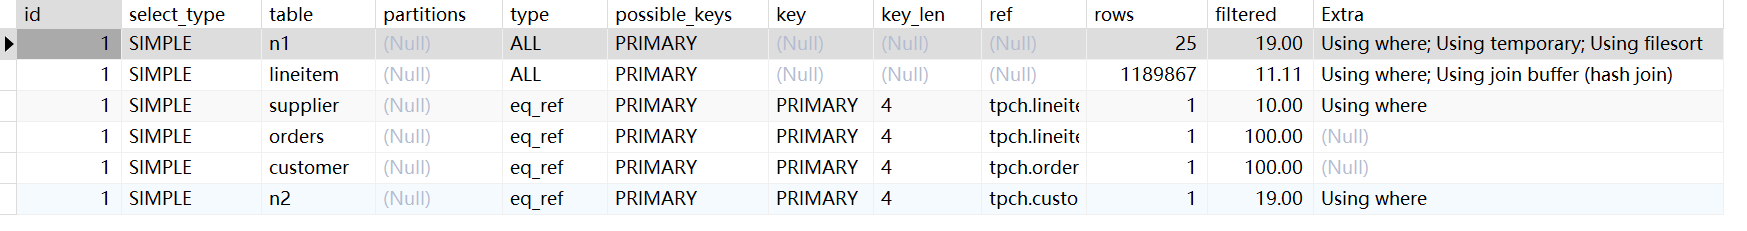
\includegraphics[width=0.9\textwidth]{img/13.png}
\caption{Q7查询 \tt{EXPLAIN} 结果}
\end{figure}

\begin{figure}[H]
\centering
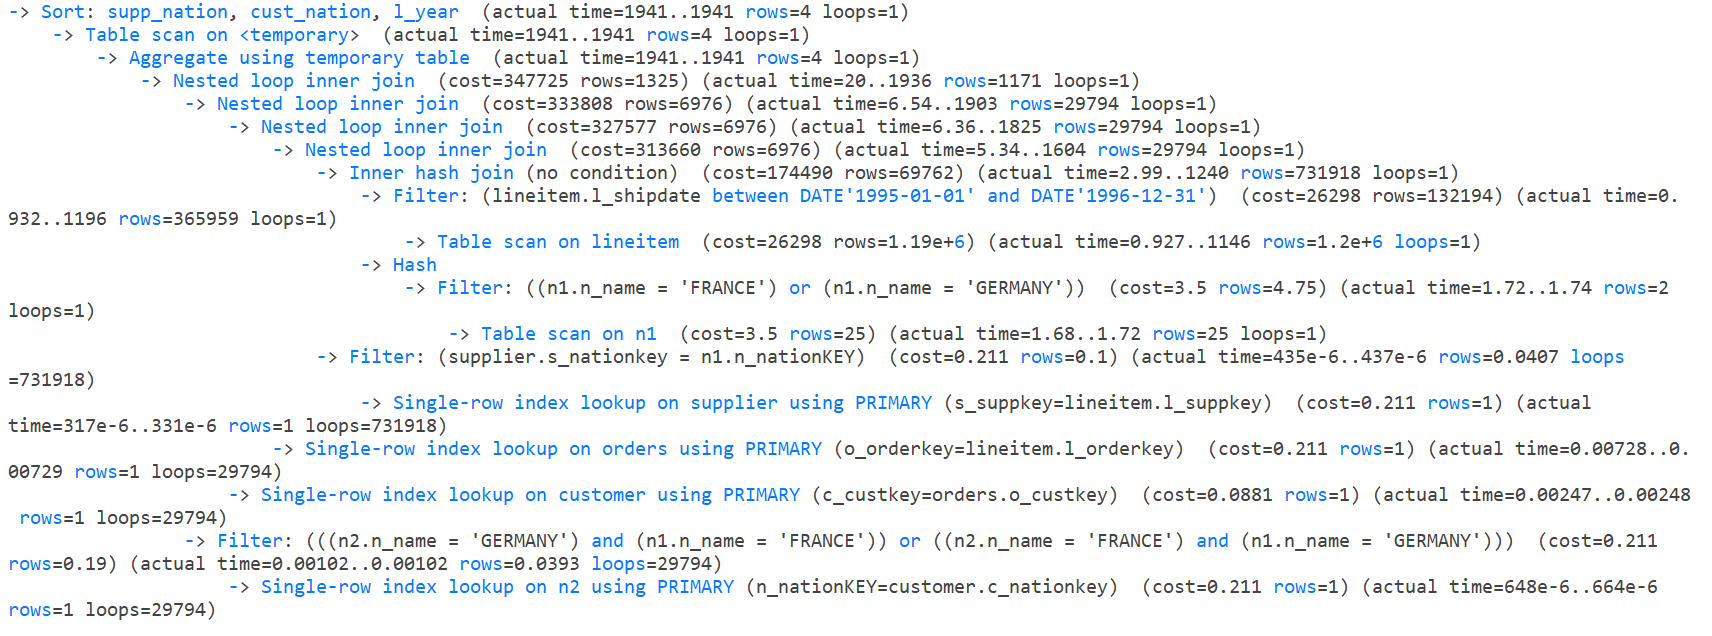
\includegraphics[width=0.9\textwidth]{img/14.png}
\caption{Q7查询 \tt{EXPLAIN ANALYZE} 结果}
\end{figure}

\begin{figure}[H]
  \centering
  \resizebox{\textwidth}{!}{
    \begin{forest}
    for tree={
      grow=south,
      draw,
      rounded corners,
      edge={->},
      node options={align=center, text width=15em}
    }
    [Sort: \tt{supp\_nation, cust\_nation, l\_year}
        [Table scan on \tt{<temporary>}
            [Aggregate using temporary table
                [Nested loop inner join
                    [Nested loop inner join
                        [Nested loop inner join
                            [Nested loop inner join
                                [Inner hash join (no condition)
                                    [Filter
                                        [Table scan on \tt{lineitem}]
                                    ]
                                    [Hash
                                        [Filter
                                            [Table scan on \tt{n1}]
                                        ]
                                    ]
                                ]
                                [Filter
                                    [Single-row index lookup on \tt{supplier} using PRIMARY (\tt{s\_suppkey=lineitem.l\_suppkey})]
                                ]
                            ]
                            [Single-row index lookup on \tt{orders} using PRIMARY (\tt{o\_orderkey=lineitem.l\_orderkey})]
                        ]
                        [Single-row index lookup on \tt{customer} using PRIMARY (\tt{c\_custkey=orders.o\_custkey})]
                    ]
                    [Filter
                        [Single-row index lookup on \tt{n2} using PRIMARY (\tt{n\_nationKEY=customer.c\_nationkey})]
                    ]
                ]
            ]
        ]
    ]
    \end{forest}
  }
  \caption{Q7查询执行计划}
\end{figure}

可以看到,Q7查询的执行计划中,对 \tt{nation} 和 \tt{lineitem} 表进行了全表扫描,没有使用索引,导致查询性能较差。可以通过为 \tt{nation} 和 \tt{lineitem} 表的相关字段创建索引来优化查询性能。

通过比较 \tt{cost} 可以发现,在扫描 \tt{lineitem} 表时,\tt{cost} 较高,因此应优先优化 \tt{lineitem} 表的查询性能。

\item Q8

\begin{lstlisting}[language=sql]
SELECT
	o_year,
	sum( CASE WHEN nation = 'BRAZIL' THEN volume ELSE 0 END ) / sum( volume ) AS mkt_share 
FROM (
	SELECT
		extract( YEAR FROM o_orderdate ) AS o_year,
		l_extendedprice * ( 1-l_discount ) AS volume, n2.n_name AS nation 
	FROM
		part, supplier, lineitem, orders, customer, nation n1, nation n2, region 
	WHERE
		p_partkey = l_partkey AND s_suppkey = l_suppkey AND l_orderkey = o_orderkey 
		AND o_custkey = c_custkey AND c_nationkey = n1.n_nationkey AND n1.n_regionkey = r_regionkey 
		AND r_name = 'AMERICA' AND s_nationkey = n2.n_nationkey 
		AND o_orderdate BETWEEN DATE '1995-01-01' AND DATE '1996-12-31' 
		AND p_type = 'ECONOMY ANODIZED STEEL' 
) AS all_nations 
GROUP BY o_year 
ORDER BY o_year;
\end{lstlisting}

\begin{figure}[H]
\centering
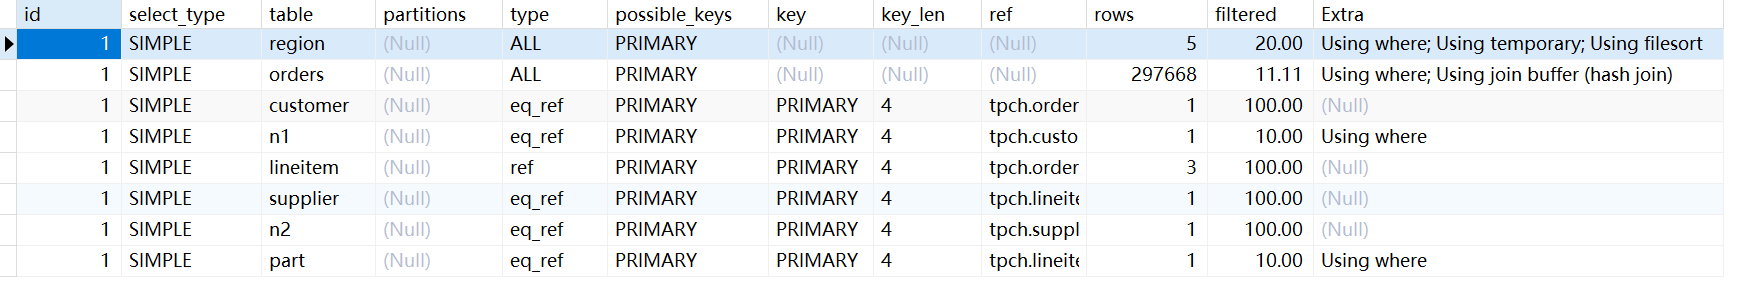
\includegraphics[width=0.9\textwidth]{img/15.png}
\caption{Q8查询 \tt{EXPLAIN} 结果}
\end{figure}

\begin{figure}[H]
\centering
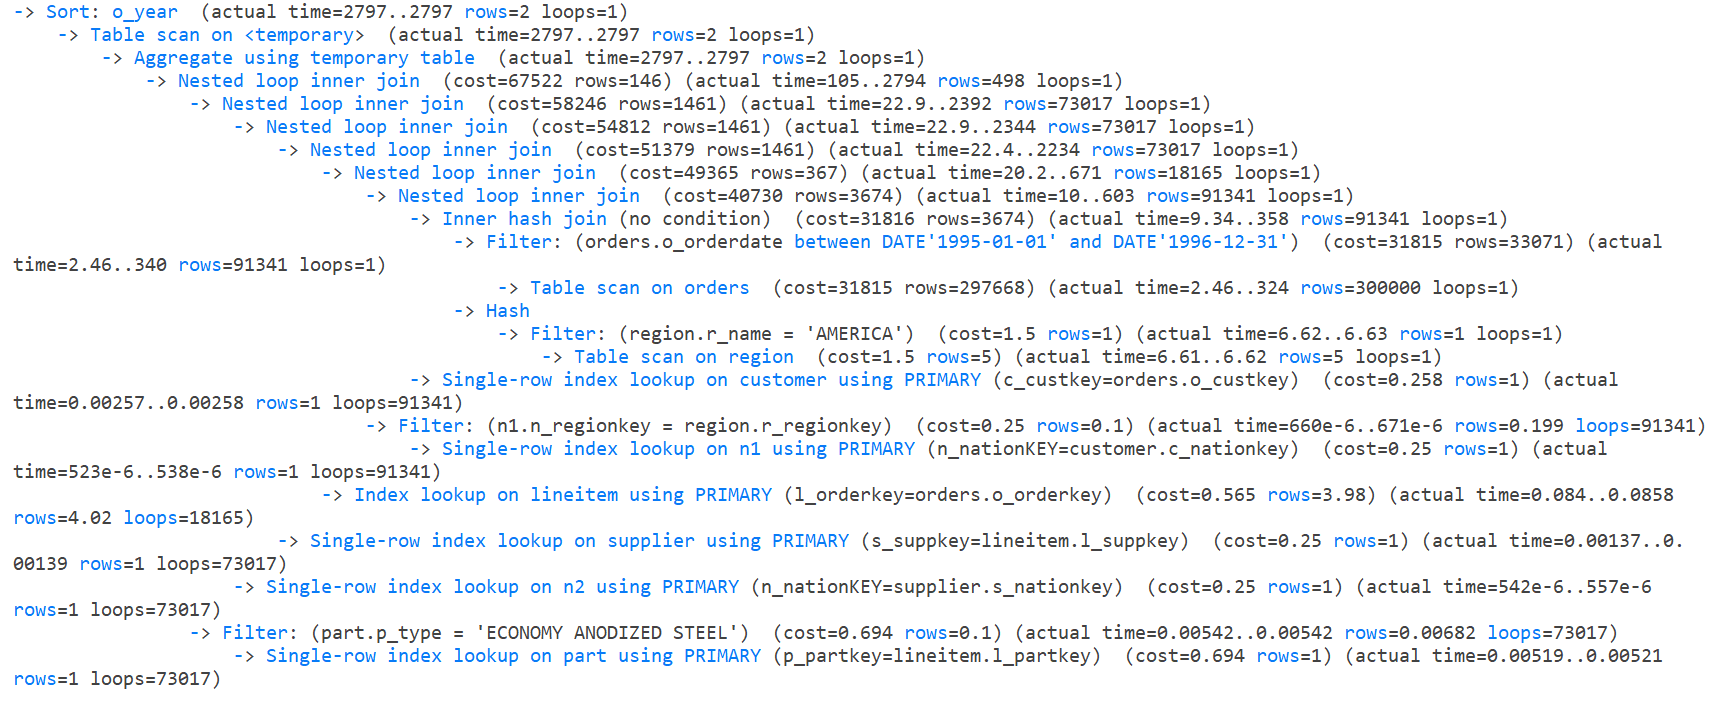
\includegraphics[width=0.9\textwidth]{img/16.png}
\caption{Q8查询 \tt{EXPLAIN ANALYZE} 结果}
\end{figure}

\begin{figure}[H]
  \centering
  \resizebox{\textwidth}{!}{
    \begin{forest}
    for tree={
      grow=south,
      draw,
      rounded corners,
      edge={->},
      node options={align=center, text width=15em}
    }
    [Sort: \tt{o\_year}
        [Table scan on \tt{<temporary>}
            [Aggregate using temporary table
                [Nested loop inner join
                    [Nested loop inner join
                        [Nested loop inner join
                            [Nested loop inner join
                                [Nested loop inner join
                                    [Nested loop inner join
                                        [Inner hash join (no condition)
                                            [Filter
                                                [Table scan on \tt{orders}]
                                            ]
                                            [Hash
                                                [Filter
                                                    [Table scan on \tt{region}]
                                                ]
                                            ]
                                        ]
                                        [Single-row index lookup on \tt{customer} using PRIMARY (\tt{c\_custkey=orders.o\_custkey})]
                                    ]
                                    [Filter
                                        [Single-row index lookup on \tt{n1} using PRIMARY (\tt{n\_nationKEY=customer.c\_nationkey})]
                                    ]
                                ]
                                [Index lookup on \tt{lineitem} using PRIMARY (\tt{l\_orderkey=orders.o\_orderkey})]
                            ]
                            [Single-row index lookup on \tt{supplier} using PRIMARY (\tt{s\_suppkey=lineitem.l\_suppkey})]
                        ]
                        [Single-row index lookup on \tt{n2} using PRIMARY (\tt{n\_nationKEY=supplier.s\_nationkey})]
                    ]
                    [Filter
                        [Single-row index lookup on \tt{part} using PRIMARY (\tt{p\_partkey=lineitem.l\_partkey})]
                    ]
                ]
            ]
        ]
    ]
    \end{forest}
  }
  \caption{Q8查询执行计划}
\end{figure}

可以看到,Q8查询的执行计划中,对 \tt{region}和 \tt{orders} 表进行了全表扫描,没有使用索引,导致查询性能较差。可以通过为 \tt{region}和 \tt{orders} 表的相关字段创建索引来优化查询性能。

通过比较 \tt{cost} 可以发现,在扫描 \tt{orders} 表时,\tt{cost} 较高,因此应优先优化 \tt{orders} 表的查询性能。

\item Q9
\begin{lstlisting}[language=sql]
select nation, o_year, sum(amount) as sum_profit 
from ( 
  select n_name as nation, extract(year from o_orderdate) as o_year, 
  l_extendedprice * (1 - l_discount) - ps_supplycost * l_quantity as amount 
  from part, supplier, lineitem, partsupp, orders, nation 
  where 
  s_suppkey = l_suppkey and ps_suppkey = l_suppkey and ps_partkey = l_partkey 
  and p_partkey = l_partkey and o_orderkey = l_orderkey and s_nationkey = n_nationkey 
  and p_name like '%green%' 
) as profit 
group by nation, o_year 
order by nation, o_year desc;
\end{lstlisting}

\begin{figure}[H]
\centering
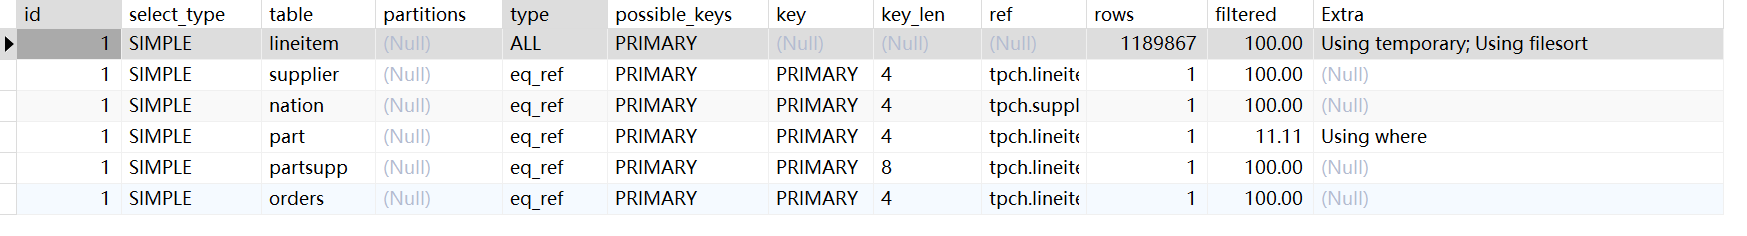
\includegraphics[width=1\textwidth]{img/17.png}
\caption{Q9查询 \tt{EXPLAIN} 结果}
\end{figure}

\begin{figure}[H]
\centering
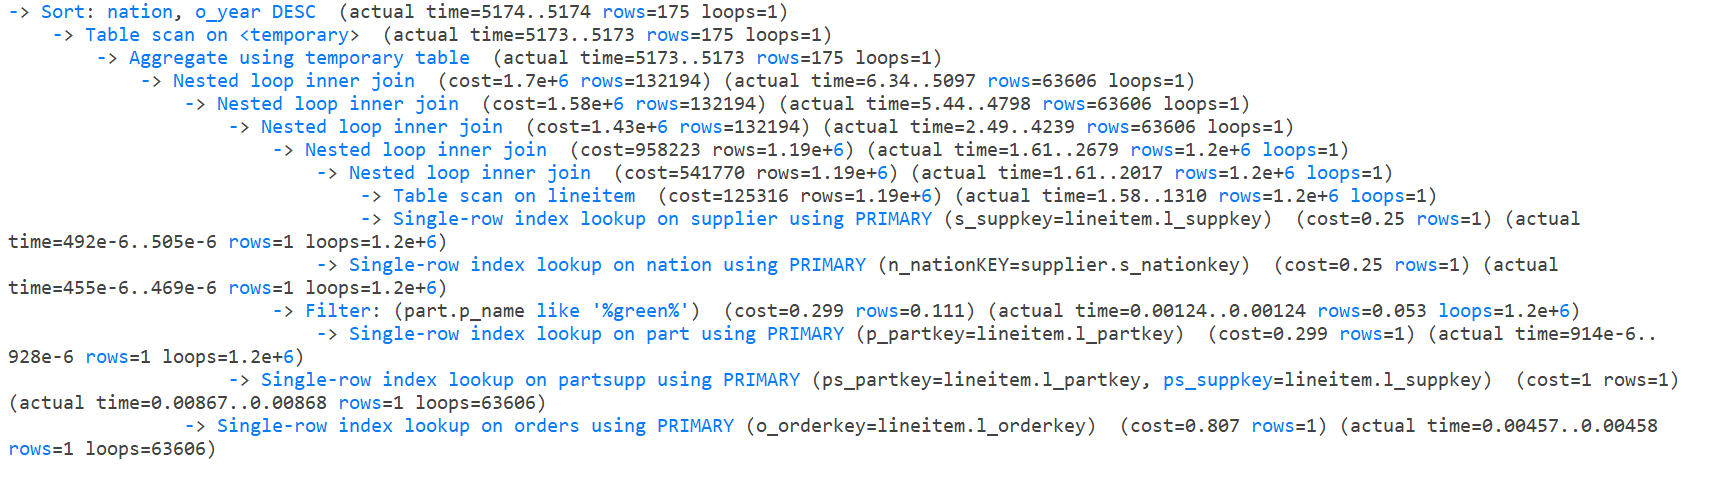
\includegraphics[width=1\textwidth]{img/18.png}
\caption{Q9查询 \tt{EXPLAIN ANALYZE} 结果}
\end{figure}

\begin{figure}[H]
  \centering
  \resizebox{\textwidth}{!}{
    \begin{forest}
    for tree={
      grow=south,
      draw,
      rounded corners,
      edge={->},
      node options={align=center, text width=15em}
    }
    [Sort: \tt{nation, o\_year DESC}
        [Table scan on \tt{<temporary>}
            [Aggregate using temporary table
                [Nested loop inner join
                    [Nested loop inner join
                        [Nested loop inner join
                            [Nested loop inner join
                                [Nested loop inner join
                                    [Table scan on \tt{lineitem}]
                                    [Single-row index lookup on \tt{supplier} using PRIMARY (\tt{s\_suppkey=lineitem.l\_suppkey})]
                                ]
                                [Single-row index lookup on \tt{nation} using PRIMARY (\tt{n\_nationKEY=supplier.s\_nationkey})]
                            ]
                            [Filter
                                [Single-row index lookup on \tt{part} using PRIMARY (\tt{p\_partkey=lineitem.l\_partkey})]
                            ]
                        ]
                        [Single-row index lookup on \tt{partsupp} using PRIMARY (\tt{ps\_partkey=lineitem.l\_partkey, ps\_suppkey=lineitem.l\_suppkey})]
                    ]
                    [Single-row index lookup on \tt{orders} using PRIMARY (\tt{o\_orderkey=lineitem.l\_orderkey})]
                ]
            ]
        ]
    ]
    \end{forest}
  }
  \caption{Q9查询执行计划}
\end{figure}

可以看到,Q9查询的执行计划中,对 \tt{lineitem} 表进行了全表扫描,没有使用索引,导致查询性能较差。可以通过为 \tt{lineitem} 表的相关字段创建索引来优化查询性能。

\item Q10

\begin{lstlisting}[language=sql]
select c_custkey, c_name, sum(l_extendedprice * (1 - l_discount)) as revenue, c_acctbal, n_name, c_address, c_phone, c_comment 
from customer, orders, lineitem, nation 
where 
	c_custkey = o_custkey and l_orderkey = o_orderkey 
	and o_orderdate >= date '1993-10-01' and o_orderdate < date '1993-10-01' + interval '3' month 
	and l_returnflag = 'R' and c_nationkey = n_nationkey 
group by c_custkey, c_name, c_acctbal, c_phone, n_name, c_address, c_comment 
order by revenue desc;
\end{lstlisting}

\begin{figure}[H]
\centering
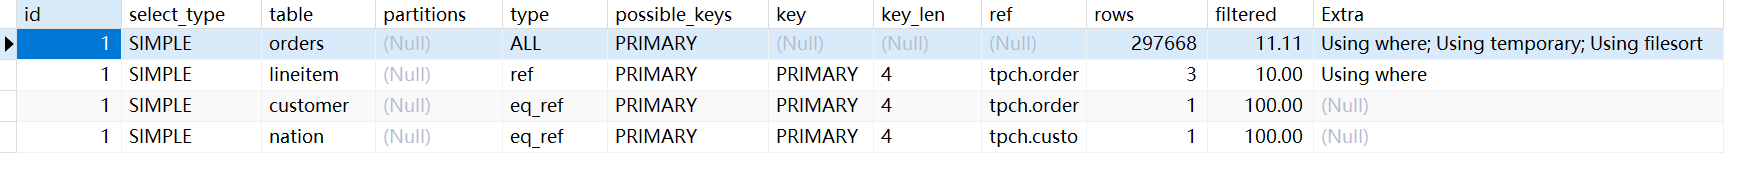
\includegraphics[width=1\textwidth]{img/19.png}
\caption{Q10查询 \tt{EXPLAIN} 结果}
\end{figure}

\begin{figure}[H]
\centering
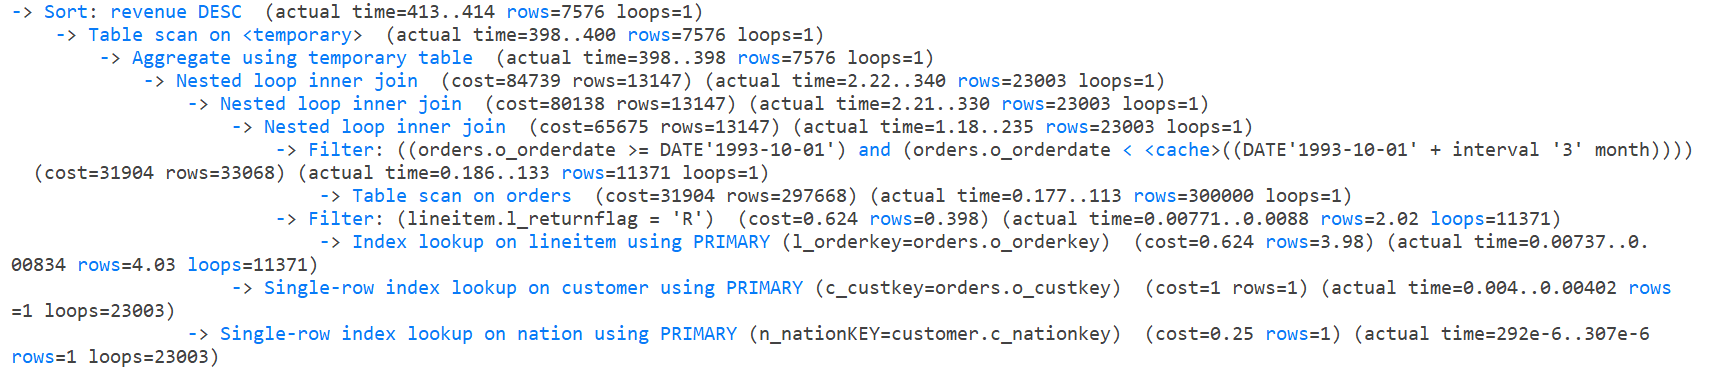
\includegraphics[width=1\textwidth]{img/20.png}
\caption{Q10查询 \tt{EXPLAIN ANALYZE} 结果}
\end{figure}
\begin{figure}[H]
  \centering
  \resizebox{\textwidth}{!}{
    \begin{forest}
    for tree={
      grow=south,
      draw,
      rounded corners,
      edge={->},
      node options={align=center, text width=15em}
    }
    [Sort: \tt{revenue DESC}
        [Table scan on \tt{<temporary>}
            [Aggregate using temporary table
                [Nested loop inner join
                    [Nested loop inner join
                        [Nested loop inner join
                            [Filter
                                [Table scan on \tt{orders}]
                            ]
                            [Filter
                                [Index lookup on \tt{lineitem} using PRIMARY (\tt{l\_orderkey=orders.o\_orderkey})]
                            ]
                        ]
                        [Single-row index lookup on \tt{customer} using PRIMARY (\tt{c\_custkey=orders.o\_custkey})]
                    ]
                    [Single-row index lookup on \tt{nation} using PRIMARY (\tt{n\_nationKEY=customer.c\_nationkey})]
                ]
            ]
        ]
    ]
    \end{forest}
  }
  \caption{Q10查询执行计划}
\end{figure}

可以看到,Q10查询的执行计划中,对 \tt{orders} 表进行了全表扫描,没有使用索引,导致查询性能较差。可以通过为 \tt{orders} 表的相关字段创建索引来优化查询性能。对\tt{orders} 表进行扫描时,\tt{cost} 较高也说明了这一点。

\item Q11

\begin{lstlisting}[language=sql]
select ps_partkey, sum(ps_supplycost * ps_availqty) as value 
from partsupp, supplier, nation 
where 
  ps_suppkey = s_suppkey and s_nationkey = n_nationkey
  and n_name = 'GERMANY' 
group by ps_partkey 
having sum(ps_supplycost * ps_availqty) > (
  select sum(ps_supplycost * ps_availqty) * 0.0001 
  from partsupp, supplier, nation 
  where ps_suppkey = s_suppkey and s_nationkey = n_nationkey and n_name = 'GERMANY' 
)
order by value desc;
\end{lstlisting}

\begin{figure}[H]
\centering
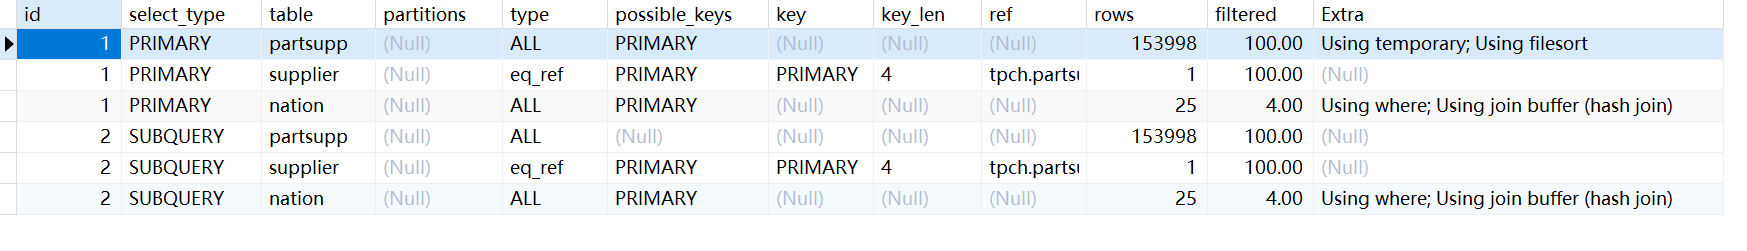
\includegraphics[width=1\textwidth]{img/21.png}
\caption{Q11查询 \tt{EXPLAIN} 结果}
\end{figure}

\begin{figure}[H]
\centering
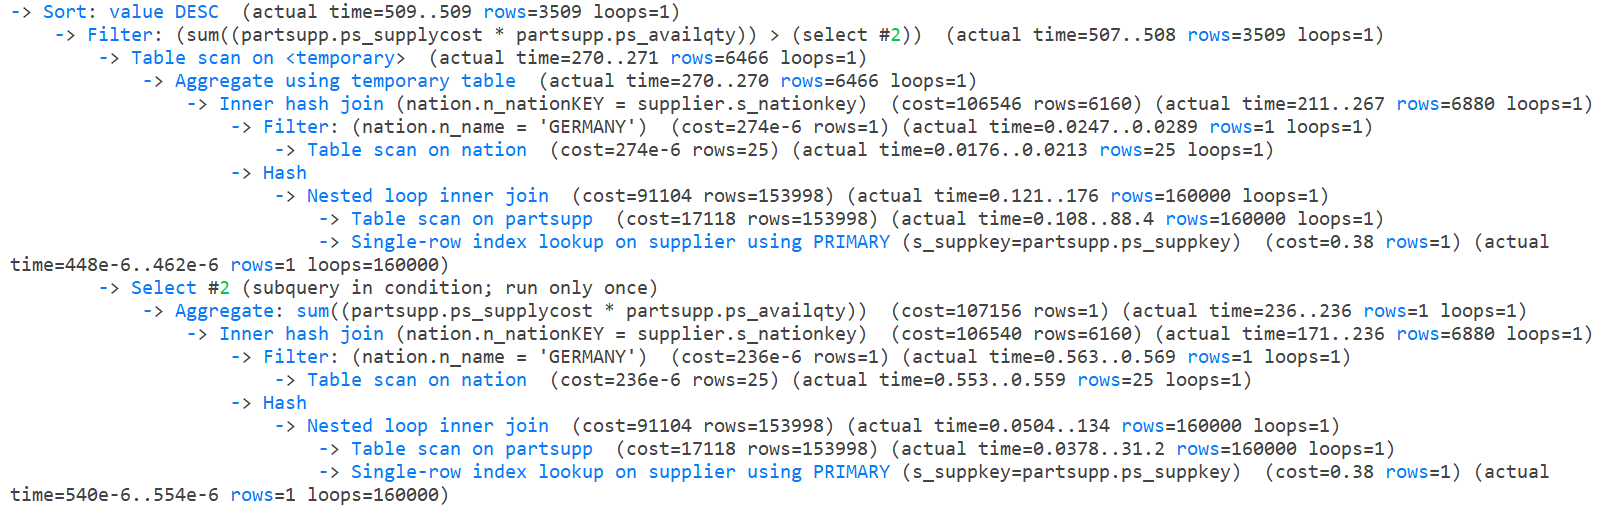
\includegraphics[width=1\textwidth]{img/22.png}
\caption{Q11查询 \tt{EXPLAIN ANALYZE} 结果}
\end{figure}

\begin{figure}[H]
  \centering
  \resizebox{\textwidth}{!}{
    \begin{forest}
    for tree={
      grow=south,
      draw,
      rounded corners,
      edge={->},
      node options={align=center, text width=20em}
    }
    [Sort: \tt{value DESC}
        [Filter: \tt{sum((partsupp.ps\_supplycost * partsupp.ps\_availqty)) > (select \#2)}
            [Table scan on \tt{<temporary>}
                [Aggregate using temporary table
                    [Inner hash join (\tt{nation.n\_nationKEY = supplier.s\_nationkey})
                        [Filter: \tt{nation.n\_name = 'GERMANY'}
                            [Table scan on \tt{nation}]
                        ]
                        [Hash
                            [Nested loop inner join
                                [Table scan on \tt{partsupp}]
                                [Single-row index lookup on \tt{supplier} using PRIMARY (\tt{s\_suppkey=partsupp.ps\_suppkey})]
                            ]
                        ]
                    ]
                ]
            ]
            [Select \#2 (subquery in condition; run only once)
                [Aggregate: \tt{sum((partsupp.ps\_supplycost * partsupp.ps\_availqty))}
                    [Inner hash join (\tt{nation.n\_nationKEY = supplier.s\_nationkey})
                        [Filter: \tt{nation.n\_name = 'GERMANY'}
                            [Table scan on \tt{nation}]
                        ]
                        [Hash
                            [Nested loop inner join
                                [Table scan on \tt{partsupp}]
                                [Single-row index lookup on \tt{supplier} using PRIMARY (\tt{s\_suppkey=partsupp.ps\_suppkey})]
                            ]
                        ]
                    ]
                ]
            ]
        ]
    ]
    \end{forest}
  }
  \caption{Q11查询执行计划}
\end{figure}

可以看到,Q11查询的执行计划中,对 \tt{partsupp},\tt{supplier} 和 \tt{nation} 表进行了全表扫描,没有使用索引,导致查询性能较差。可以通过为 \tt{partsupp},\tt{supplier} 和 \tt{nation} 表的相关字段创建索引来优化查询性能。

通过比较 \tt{cost} 可以发现,在扫描 \tt{partsupp} 表时,\tt{cost} 较高,因此应优先优化 \tt{partsupp} 表的查询性能。

\item Q12

\begin{lstlisting}[language=sql]
select l_shipmode, sum(
		case when o_orderpriority ='1-URGENT' or o_orderpriority ='2-HIGH' then 1 else 0 end
	) as high_line_count, sum(
		case when o_orderpriority <> '1-URGENT' and o_orderpriority <> '2-HIGH' then 1 else 0 end
	) as low_line_count 
from orders, lineitem 
where 
	o_orderkey = l_orderkey and l_shipmode in ('MAIL', 'SHIP') and l_commitdate < l_receiptdate 
	and l_shipdate < l_commitdate and l_receiptdate >= date '1994-01-01' 
	and l_receiptdate < date '1994-01-01' + interval '1' year 
group by l_shipmode
order by l_shipmode;
\end{lstlisting}

\begin{figure}[H]
\centering
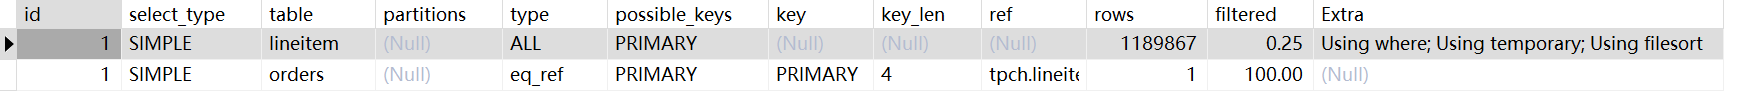
\includegraphics[width=1\textwidth]{img/23.png}
\caption{Q12查询 \tt{EXPLAIN} 结果}
\end{figure}

\begin{figure}[H]
\centering
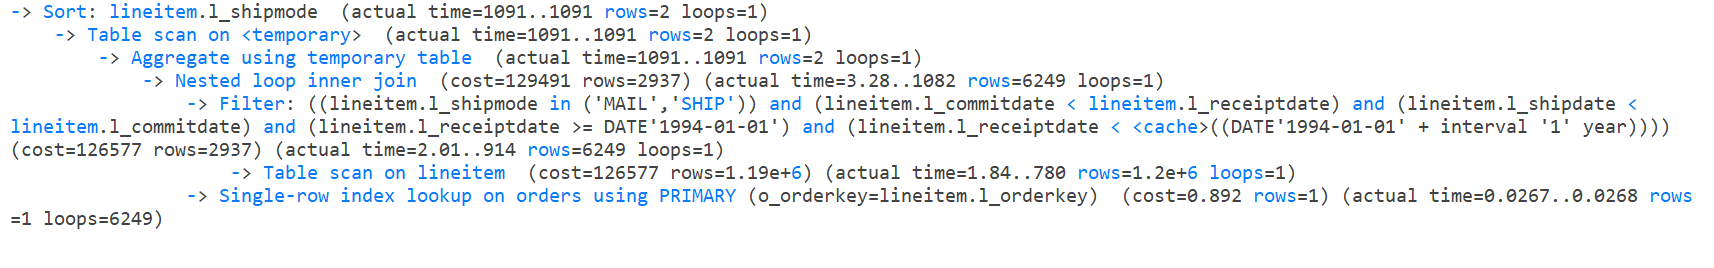
\includegraphics[width=1\textwidth]{img/24.png}
\caption{Q12查询 \tt{EXPLAIN ANALYZE} 结果}
\end{figure}

\begin{figure}[H]
  \centering
  \resizebox{0.8\textwidth}{!}{
    \begin{forest}
    for tree={
      grow=south,
      draw,
      rounded corners,
      edge={->},
      node options={align=center, text width=20em}
    }
    [Sort: \tt{lineitem.l\_shipmode}
        [Filter
            [Table scan on \tt{<temporary>}
                [Aggregate using temporary table
                    [Nested loop inner join
                        [Filter: \tt{lineitem.l\_shipmode in ('MAIL','SHIP')}
                            [Table scan on \tt{lineitem}]
                        ]
                        [Single-row index lookup on \tt{orders} using PRIMARY (\tt{o\_orderkey=lineitem.l\_orderkey})]
                    ]
                ]
            ]
        ]
    ]
    \end{forest}
  }
  \caption{Q12查询执行计划}
\end{figure}

可以看到,Q12查询的执行计划中,对 \tt{lineitem} 表进行了全表扫描,没有使用索引,导致查询性能较差。可以通过为 \tt{lineitem} 表的相关字段创建索引来优化查询性能。对\tt{lineitem} 表进行扫描时,\tt{cost} 较高也说明了这一点。

\item Q13

\begin{lstlisting}[language=sql]
select c_count, count(*) as custdist 
from ( 
  select c_custkey, count(o_orderkey) from customer 
  left outer join orders on c_custkey = o_custkey and o_comment not like '%special%requests%' 
  group by c_custkey
) as c_orders(c_custkey, c_count) 
group by c_count 
order by custdist desc, c_count desc;
\end{lstlisting}

\begin{figure}[H]
\centering
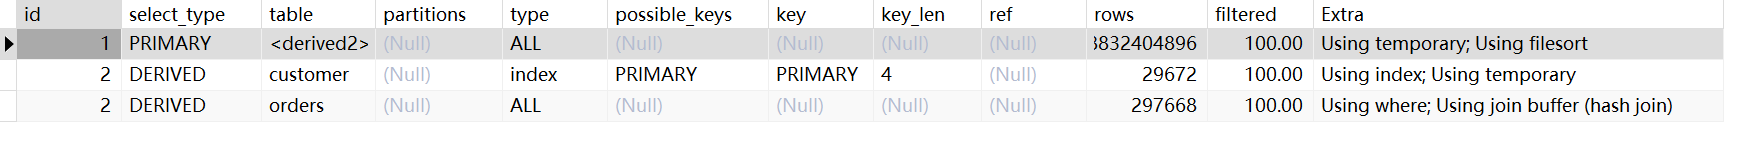
\includegraphics[width=1\textwidth]{img/25.png}
\caption{Q13查询 \tt{EXPLAIN} 结果}
\end{figure}

\begin{figure}[H]
\centering
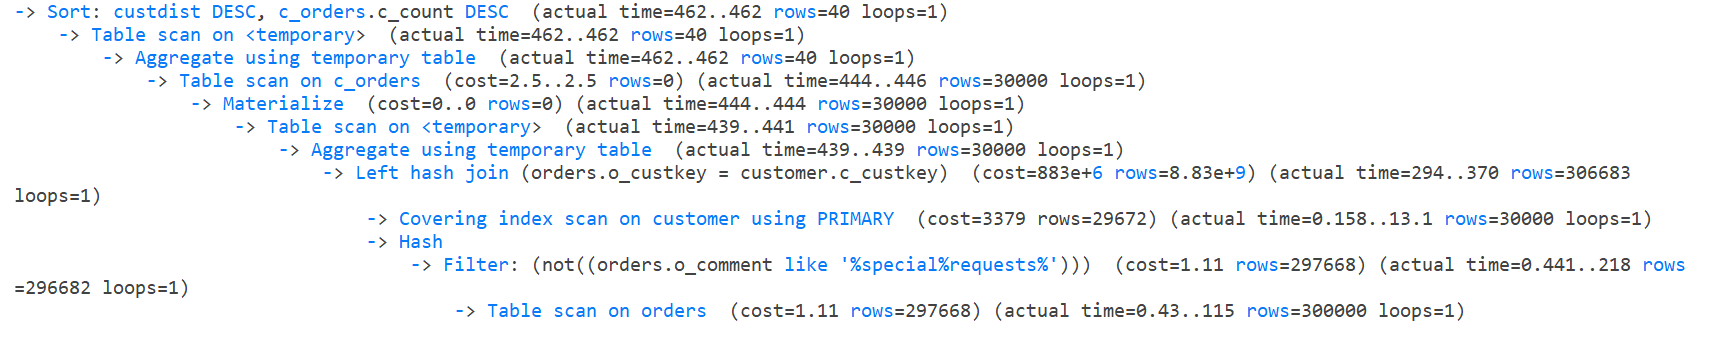
\includegraphics[width=1\textwidth]{img/26.png}
\caption{Q13查询 \tt{EXPLAIN ANALYZE} 结果}
\end{figure}

\begin{figure}[H]
  \centering
  \resizebox{0.6\textwidth}{!}{
    \begin{forest}
    for tree={
      grow=south,
      draw,
      rounded corners,
      edge={->},
      node options={align=center, text width=20em}
    }
    [Sort: \tt{custdist DESC, c\_orders.c\_count DESC}
        [Table scan on \tt{<temporary>}
            [Aggregate using temporary table
                [Table scan on \tt{c\_orders} 
                    [Materialize
                        [Table scan on \tt{<temporary>} 
                            [Aggregate using temporary table 
                                [Left hash join (orders.o\_custkey = customer.c\_custkey)
                                    [Covering index scan on customer using PRIMARY]
                                    [Hash
                                        [Filter: \tt{not((orders.o\_comment like '\%special\%requests\%'))}
                                            [Table scan on \tt{orders}]
                                        ]
                                    ]
                                ]
                            ]
                        ]
                    ]
                ]
            ]
        ]
    ]
    \end{forest}
  }
  \caption{Q13查询执行计划}
\end{figure}

可以看到,Q13查询的执行计划中,对 \tt{orders} 表进行了全表扫描,没有使用索引,导致查询性能较差。可以通过为 \tt{orders} 表的相关字段创建索引来优化查询性能。\tt{orders} 参与\tt{LEFT JOIN} 时,\tt{cost} 很高也说明了这一点。 

\item Q14

\begin{lstlisting}[language=sql]
select 100.00 * sum(
		case when p_type like 'PROMO%' then l_extendedprice*(1 - l_discount) else 0 end
	) / sum(l_extendedprice * (1 - l_discount)) as promo_revenue 
from lineitem, part 
where l_partkey = p_partkey and l_shipdate >= date '1995-09-01' 
	and l_shipdate < date '1995-09-01' + interval '1' month;
\end{lstlisting}

\begin{figure}[H]
\centering
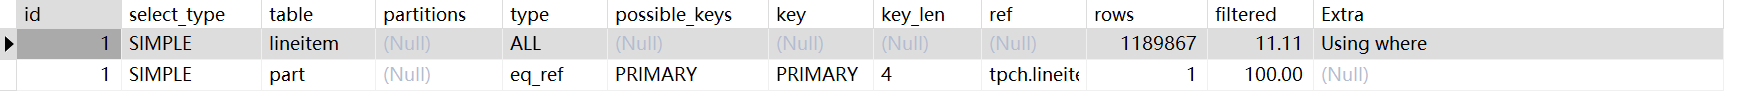
\includegraphics[width=1\textwidth]{img/27.png}
\caption{Q14查询 \tt{EXPLAIN} 结果}
\end{figure}

\begin{figure}[H]
\centering
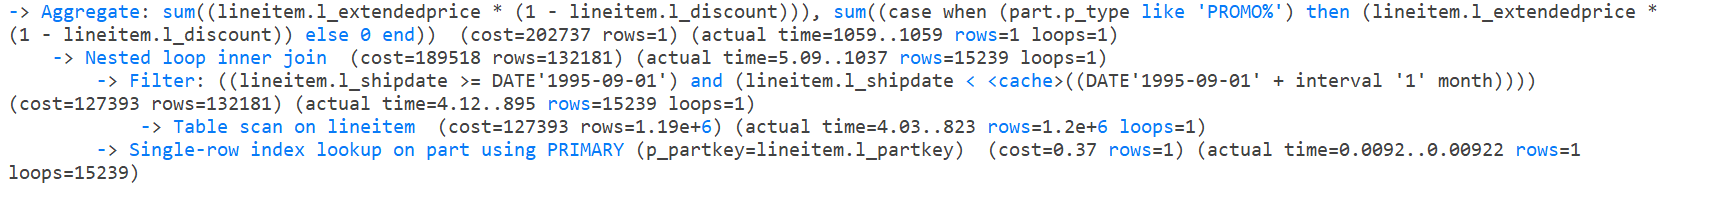
\includegraphics[width=1\textwidth]{img/28.png}
\caption{Q14查询 \tt{EXPLAIN ANALYZE} 结果}
\end{figure}

\begin{figure}[H]
  \centering
  \resizebox{0.7\textwidth}{!}{
    \begin{forest}
    for tree={
      grow=south,
      draw,
      rounded corners,
      edge={->},
      node options={align=center, text width=20em}
    }
    [Aggregate: \tt{sum((lineitem.l\_extendedprice * (1 - lineitem.l\_discount))),}\\ \tt{sum((case when (part.p\_type like 'PROMO\%') then (lineitem.l\_extendedprice * (1 - lineitem.l\_discount)) else 0 end))}
        [Nested loop inner join
            [Filter: \tt{((lineitem.l\_shipdate >= DATE'1995-09-01') and (lineitem.l\_shipdate < <cache>((DATE'1995-09-01' + interval '1' month))))}
                [Table scan on \tt{lineitem}]
            ]
            [Single-row index lookup on part using PRIMARY (p\_partkey=lineitem.l\_partkey)]
        ]
    ]
    \end{forest}
  }
  \caption{Q14查询执行计划}
\end{figure}

可以看到,Q14查询的执行计划中,对 \tt{lineitem} 表进行了全表扫描,没有使用索引,导致查询性能较差。可以通过为 \tt{lineitem} 表的相关字段创建索引来优化查询性能。对\tt{lineitem} 表进行扫描时,\tt{cost} 较高也说明了这一点。

\item Q15

\begin{lstlisting}[language=sql]
with revenue1996(supplier_no, total_revenue) as (
  select l_suppkey,
  sum(l_extendedprice * (1 - l_discount)) from lineitem 
  where l_shipdate >= date '1996-01-01' and l_shipdate < date '1996-01-01' + interval '3' month 
  group by l_suppkey
) 
select s_suppkey, s_name, s_address, s_phone, total_revenue 
from supplier, revenue1996 
where s_suppkey = supplier_no and total_revenue = (
  select max(total_revenue) from revenue1996 
) 
order by s_suppkey;
\end{lstlisting}

\begin{figure}[H]
\centering
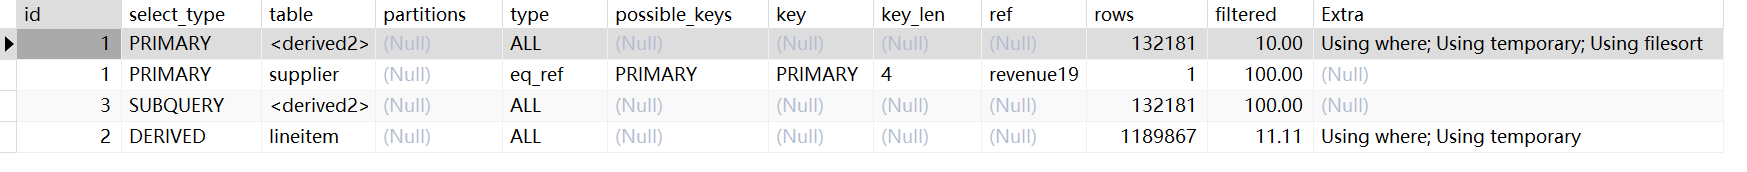
\includegraphics[width=1\textwidth]{img/29.png}
\caption{Q15查询 \tt{EXPLAIN} 结果}
\end{figure}

\begin{figure}[H]
\centering
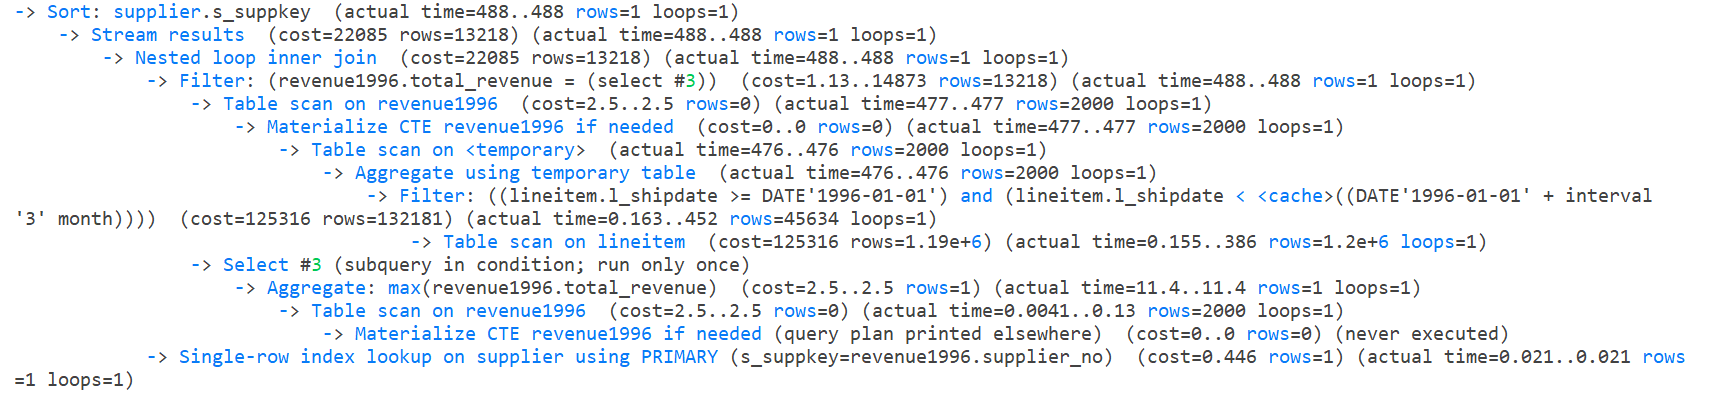
\includegraphics[width=1\textwidth]{img/30.png}
\caption{Q15查询 \tt{EXPLAIN ANALYZE} 结果}
\end{figure}

\begin{figure}[H]
  \centering
  \resizebox{\textwidth}{!}{
    \begin{forest}
    for tree={
      grow=south,
      draw,
      rounded corners,
      edge={->},
      node options={align=center, text width=20em}
    }
    [Sort: supplier.s\_suppkey
        [Stream results
            [Nested loop inner join
                [Filter: (revenue1996.total\_revenue \tt{=} (select \#3))
                    [Table scan on revenue1996
                        [Materialize CTE revenue1996 if needed
                            [Table scan on <temporary>
                                [Aggregate using temporary table
                                    [Filter
                                        [Table scan on lineitem]
                                    ]
                                ]
                            ]
                        ]
                    ]
                ]
                [Select \#3 (subquery in condition; run only once)
                    [Aggregate: max(revenue1996.total\_revenue)
                        [Table scan on revenue1996
                            [Materialize CTE revenue1996 if needed (query plan printed elsewhere)]
                        ]
                    ]
                ]
                [Single-row index lookup on supplier using PRIMARY (s\_suppkey\tt{=}revenue1996.supplier\_no)]
            ]
        ]
    ]
    \end{forest}
  }
  \caption{Q15 查询执行计划}
\end{figure}

可以看到,Q15查询的执行计划中,对 \tt{lineitem} 表进行了全表扫描,没有使用索引,导致查询性能较差。可以通过为 \tt{lineitem} 表的相关字段创建索引来优化查询性能。对\tt{lineitem} 表进行扫描时,\tt{cost} 较高也说明了这一点。

\item Q16
\begin{lstlisting}[language=sql]
select p_brand, p_type, p_size, count(distinct ps_suppkey) as supplier_cnt
from partsupp, part 
where p_partkey = ps_partkey and p_brand <> 'Brand#45'
  and p_type not like 'MEDIUM POLISHED%' and p_size in (49, 14, 23, 45, 19, 3, 36, 9) 
  and ps_suppkey not in ( 
    select s_suppkey from supplier where s_comment like '%Customer%Complaints%' 
  ) 
group by p_brand, p_type, p_size
order by supplier_cnt desc, p_brand, p_type, p_size;
\end{lstlisting}

\begin{figure}[H]
\centering

\includegraphics[width=1\textwidth]{img/31.png}
\caption{Q16查询 \tt{EXPLAIN} 结果}
\end{figure}

\begin{figure}[H]
\centering
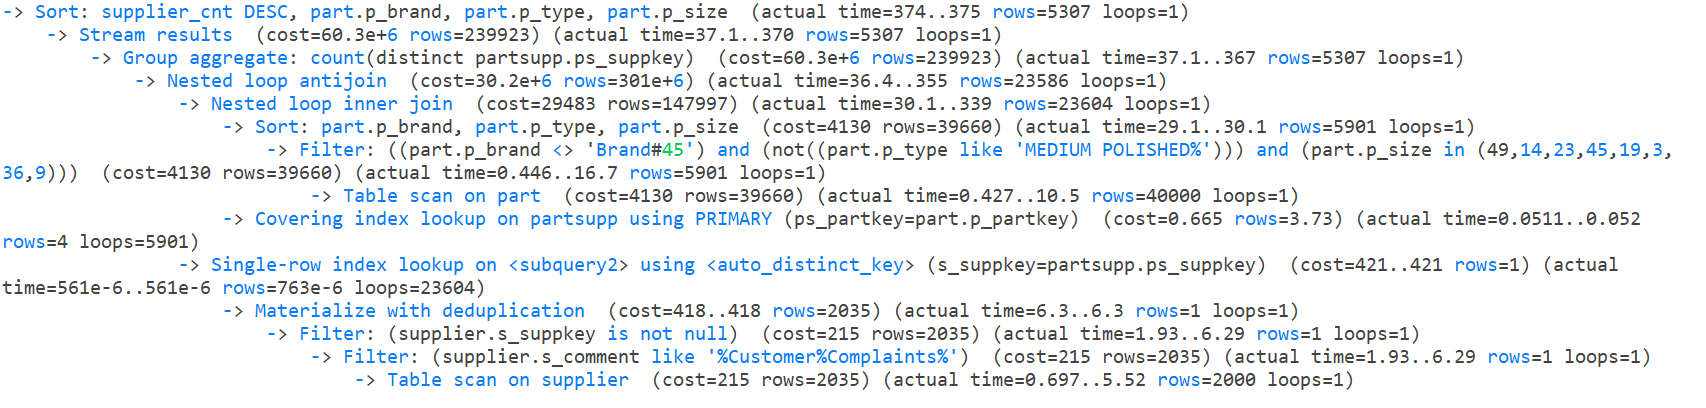
\includegraphics[width=1\textwidth]{img/32.png}
\caption{Q16查询 \tt{EXPLAIN ANALYZE} 结果}
\end{figure}

\begin{figure}[H]
  \centering
  \resizebox{\textwidth}{!}{
    \begin{forest}
    for tree={
      grow=south,
      draw,
      rounded corners,
      edge={->},
      node options={align=center, text width=20em}
    }
    [Sort: \tt{supplier\_cnt DESC, part.p\_brand, part.p\_type, part.p\_size}
        [Stream results
            [Group aggregate: count(distinct partsupp.ps\_suppkey)
                [Nested loop antijoin
                    [Nested loop inner join
                        [Sort: \tt{part.p\_brand, part.p\_type, part.p\_size}
                            [Filter
                                [Table scan on part]
                            ]
                        ]
                        [Covering index lookup on partsupp using PRIMARY (ps\_partkey\tt{=}part.p\_partkey)]
                    ]
                    [Single-row index lookup on <subquery2> using <auto\_distinct\_key> (s\_suppkey\tt{=}partsupp.ps\_suppkey)
                        [Materialize with deduplication
                            [Filter
                                [Filter
                                    [Table scan on supplier]
                                ]
                            ]
                        ]
                    ]
                ]
            ]
        ]
    ]
    \end{forest}
  }
  \caption{Q16 查询执行计划}
\end{figure}

可以看到,Q16查询的执行计划中,对 \tt{part}和 \tt{supplier} 表进行了全表扫描,没有使用索引,导致查询性能较差。可以通过为 \tt{part}和 \tt{supplier} 表的相关字段创建索引来优化查询性能。

\item Q17

\begin{lstlisting}[language=sql]
select sum(l_extendedprice) / 7.0 as avg_yearly 
from lineitem, part 
where p_partkey = l_partkey and p_brand = 'Brand#23' and p_container = 'MED BOX' 
and l_quantity < (select 0.2 * avg(l_quantity) from lineitem where l_partkey = p_partkey);
\end{lstlisting}

\begin{figure}[H]
\centering
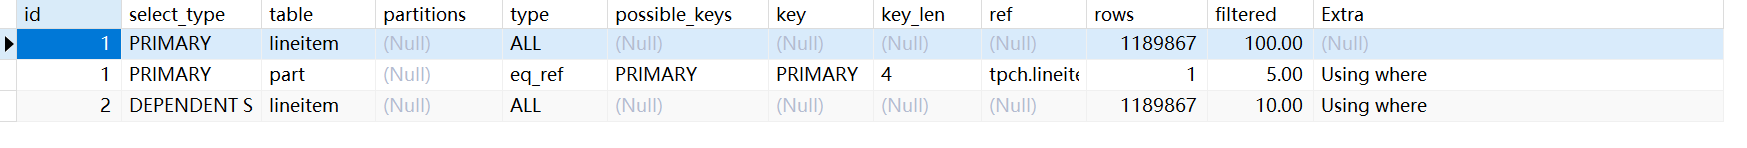
\includegraphics[width=1\textwidth]{img/33.png}
\caption{Q17查询 \tt{EXPLAIN} 结果}
\end{figure}

\begin{figure}[H]
\centering
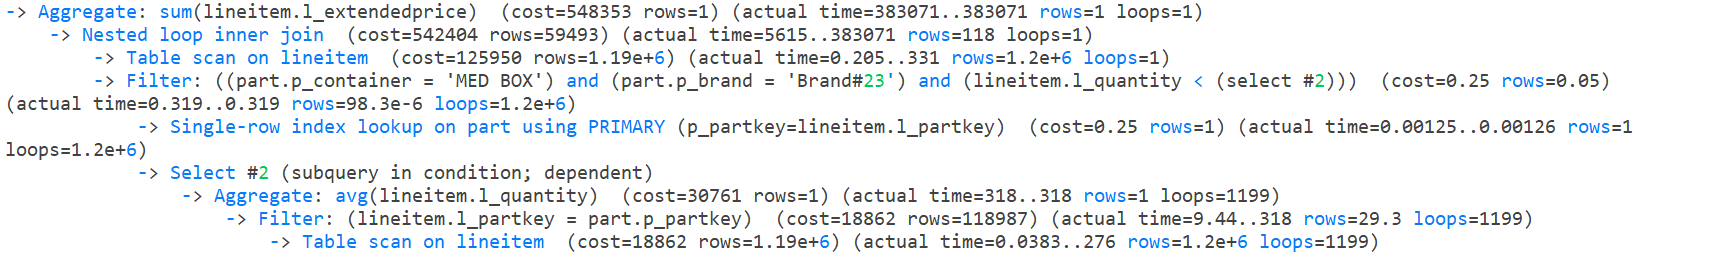
\includegraphics[width=1\textwidth]{img/34.png}
\caption{Q17查询 \tt{EXPLAIN ANALYZE} 结果}
\end{figure}

\begin{figure}[H]
  \centering
  \resizebox{\textwidth}{!}{
    \begin{forest}
    for tree={
      grow=south,
      draw,
      rounded corners,
      edge={->},
      node options={align=center, text width=25em}
    }
    [Aggregate: sum(lineitem.l\_extendedprice)
        [Nested loop inner join
            [Table scan on lineitem]
            [Filter: ((part.p\_container \tt{=} 'MED BOX') and (part.p\_brand \tt{=} 'Brand\#23') and (lineitem.l\_quantity < (select \#2)))
                [Single-row index lookup on part using PRIMARY (p\_partkey\tt{=}lineitem.l\_partkey)]
                [Select \#2 (subquery in condition; dependent)
                    [Aggregate: avg(lineitem.l\_quantity)
                        [Filter: (lineitem.l\_partkey \tt{=} part.p\_partkey)
                            [Table scan on lineitem]
                        ]
                    ]
                ]
            ]
        ]
    ]
    \end{forest}
  }
  \caption{Q17 查询执行计划}
\end{figure}

可以看到,Q17查询的执行计划中,对 \tt{lineitem} 表进行了全表扫描,没有使用索引,导致查询性能较差,用时很长。可以通过为 \tt{lineitem} 表的相关字段创建索引来优化查询性能。

\item Q18

\begin{lstlisting}[language=sql]
select c_name, c_custkey, o_orderkey, o_orderdate, o_totalprice, sum(l_quantity) 
from customer, orders, lineitem where o_orderkey in ( 
  select l_orderkey from lineitem group by l_orderkey having sum(l_quantity) > 300 
)
and c_custkey = o_custkey and o_orderkey = l_orderkey 
group by c_name, c_custkey, o_orderkey, o_orderdate, o_totalprice 
order by o_totalprice desc, o_orderdate;
\end{lstlisting}

\begin{figure}[H]
\centering
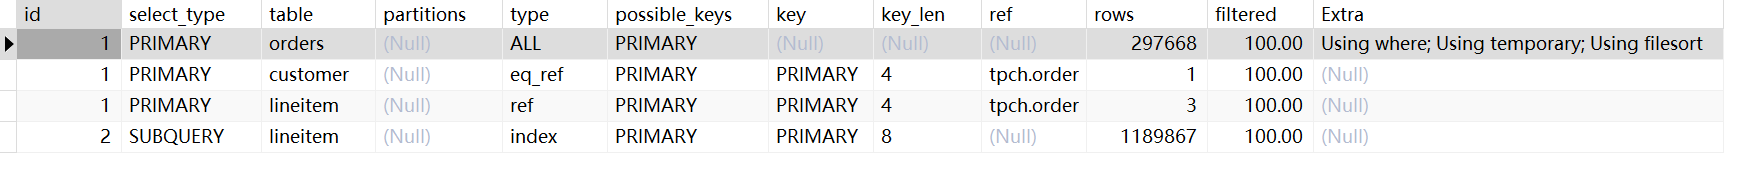
\includegraphics[width=1\textwidth]{img/35.png}
\caption{Q18查询 \tt{EXPLAIN} 结果}
\end{figure}

\begin{figure}[H]
\centering
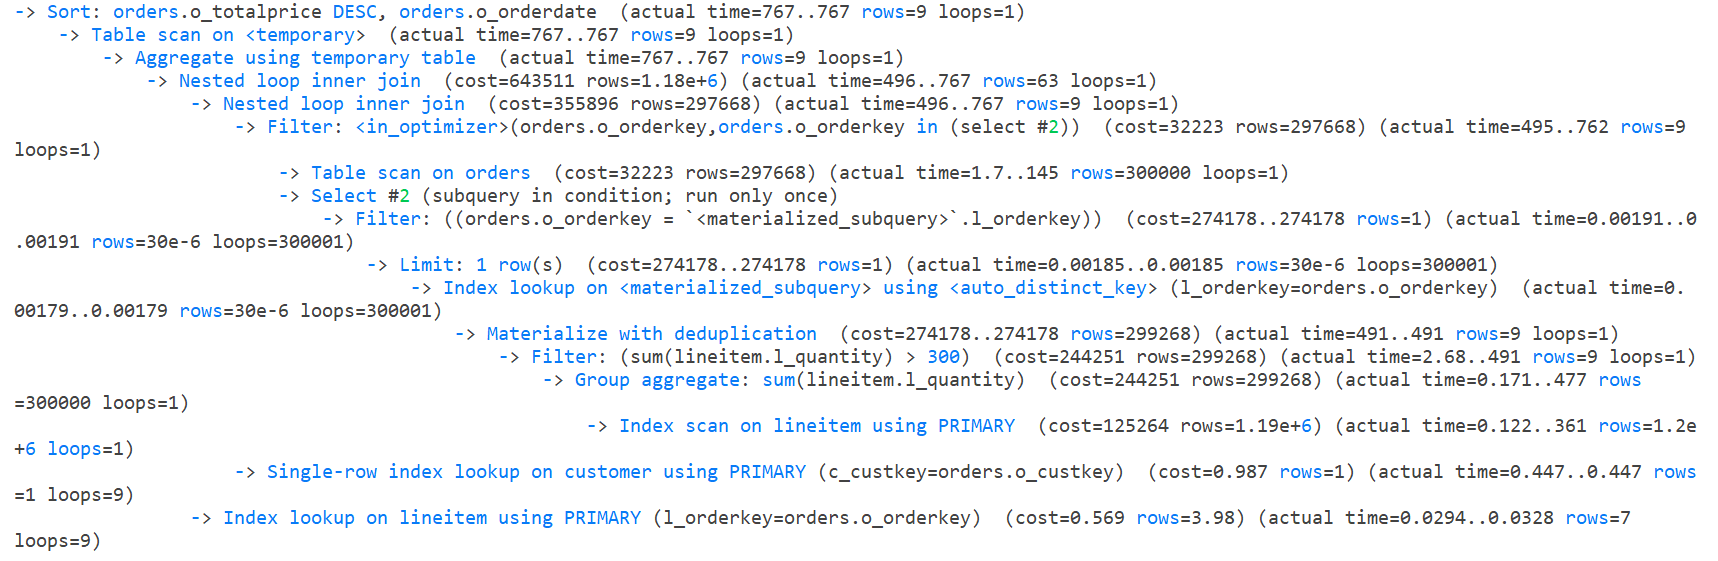
\includegraphics[width=1\textwidth]{img/36.png}
\caption{Q18查询 \tt{EXPLAIN ANALYZE} 结果}
\end{figure}

\begin{figure}[H]
  \centering
  \resizebox{\textwidth}{!}{
    \begin{forest}
    for tree={
      grow=south,
      draw,
      rounded corners,
      edge={->},
      node options={align=center, text width=15em}
    }
    [Sort: \tt{orders.o\_totalprice DESC, orders.o\_orderdate}
        [Table scan on <temporary>
            [Aggregate using temporary table
                [Nested loop inner join
                    [Nested loop inner join
                        [Filter: \tt{<in\_optimizer>(orders.o\_orderkey, orders.o\_orderkey in (select \#2))}
                            [Table scan on orders]
                            [Select \#2 (subquery in condition; run only once)
                                [Filter: \tt{((orders.o\_orderkey \tt{=} `<materialized\_subquery>`.l\_orderkey))}
                                    [Limit: 1 row(s)
                                        [Index lookup on <materialized\_subquery> using <auto\_distinct\_key> (l\_orderkey\tt{=}orders.o\_orderkey)
                                            [Materialize with deduplication
                                                [Filter: (sum(lineitem.l\_quantity) > 300)
                                                    [Group aggregate: sum(lineitem.l\_quantity)
                                                        [Index scan on lineitem using PRIMARY]
                                                    ]
                                                ]
                                            ]
                                        ]
                                    ]
                                ]
                            ]
                        ]
                        [Single-row index lookup on customer using PRIMARY (c\_custkey\tt{=}orders.o\_custkey)]
                    ]
                    [Index lookup on lineitem using PRIMARY (l\_orderkey\tt{=}orders.o\_orderkey)]
                ]
            ]
        ]
    ]
    \end{forest}
  }
  \caption{Q18 查询执行计划}
\end{figure}

可以看到,Q18查询的执行计划中,对 \tt{orders} 表进行了全表扫描,没有使用索引,导致查询性能较差。可以通过为 \tt{orders} 表的相关字段创建索引来优化查询性能。

从 \tt{cost} 上看,\tt{orders} 表和 \tt{lineitem} 表的扫描成本都比较高。

\item Q19

\begin{lstlisting}[language=sql]
SELECT
	sum( l_extendedprice * ( 1 - l_discount ) ) AS revenue 
FROM lineitem, part 
WHERE (
		p_partkey = l_partkey AND p_brand = 'Brand#12' 
		AND p_container IN ( 'SM CASE', 'SM BOX', 'SM PACK', 'SM PKG' ) 
		AND l_quantity >= 1 AND l_quantity <= 1 + 10 
		AND p_size BETWEEN 1 AND 5 AND l_shipmode IN ( 'AIR', 'AIR REG' ) 
		AND l_shipinstruct = 'DELIVER IN PERSON' 
	) OR (
		p_partkey = l_partkey AND p_brand = 'Brand#23' 
		AND p_container IN ( 'MED BAG', 'MED BOX', 'MED PKG', 'MED PACK' ) 
		AND l_quantity >= 10 AND l_quantity <= 10 + 10 
		AND p_size BETWEEN 1 AND 10 AND l_shipmode IN ( 'AIR', 'AIR REG' ) 
		AND l_shipinstruct = 'DELIVER IN PERSON' 
	) OR (
		p_partkey = l_partkey AND p_brand = 'Brand#34' 
		AND p_container IN ( 'LG CASE', 'LG BOX', 'LG PACK', 'LG PKG' ) 
		AND l_quantity >= 20 AND l_quantity <= 20 + 10 
		AND p_size BETWEEN 1 AND 15 AND l_shipmode IN ( 'AIR', 'AIR REG' ) 
		AND l_shipinstruct = 'DELIVER IN PERSON' 
);
\end{lstlisting}

\begin{figure}[H]
\centering
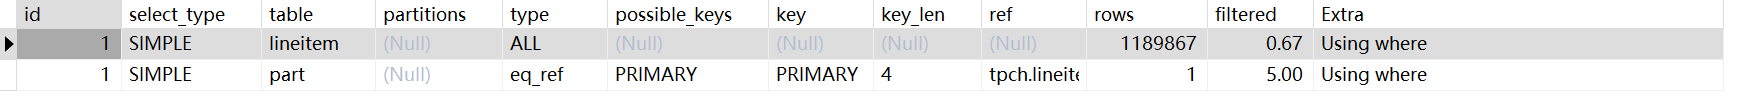
\includegraphics[width=1\textwidth]{img/37.png}
\caption{Q19查询 \tt{EXPLAIN} 结果}
\end{figure}

\begin{figure}[H]
\centering
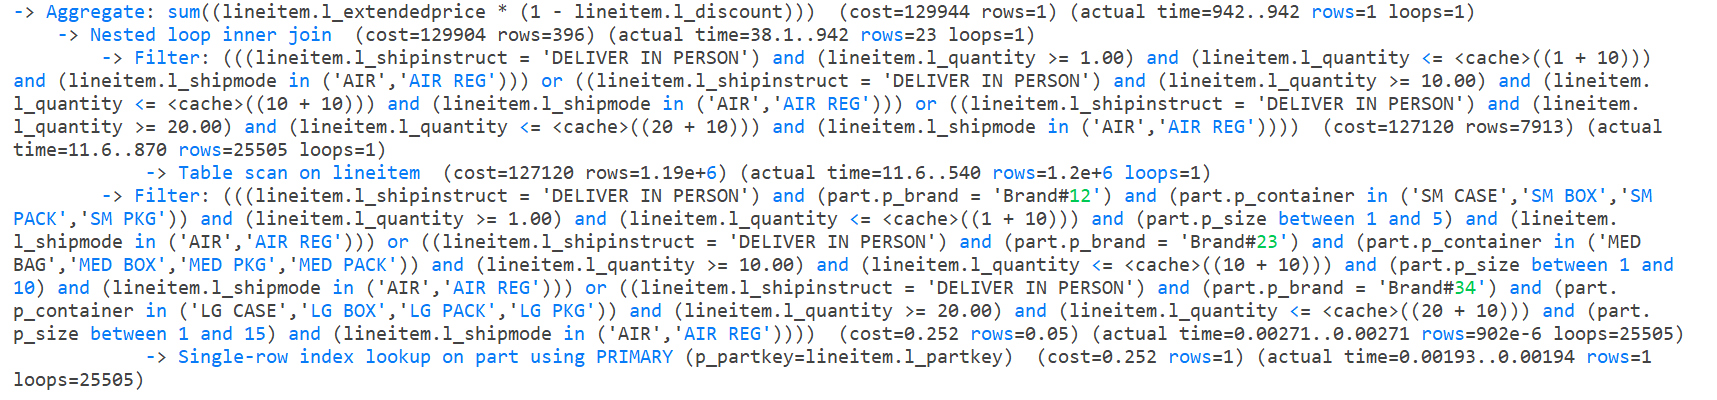
\includegraphics[width=1\textwidth]{img/38.png}
\caption{Q19查询 \tt{EXPLAIN ANALYZE} 结果}
\end{figure}

\begin{figure}[H]
  \centering
  \resizebox{\textwidth}{!}{
    \begin{forest}
    for tree={
      grow=south,
      draw,
      rounded corners,
      edge={->},
      node options={align=center, text width=25em}
    }
    [Aggregate: sum((lineitem.l\_extendedprice * (1 - lineitem.l\_discount)))
        [Nested loop inner join
            [Filter
                [Table scan on lineitem]
            ]
            [Filter
                [Single-row index lookup on part using PRIMARY (p\_partkey\tt{=}lineitem.l\_partkey)]
            ]
        ]
    ]
    \end{forest}
  }
  \caption{Q19 查询执行计划}
\end{figure}

可以看到,Q19查询的执行计划中,对 \tt{lineitem} 表进行了全表扫描,没有使用索引,导致查询性能较差。可以通过为 \tt{lineitem} 表的相关字段创建索引来优化查询性能。从 \tt{cost} 上看,\tt{lineitem} 表的扫描成本也是比较高的。

\item Q20

\begin{lstlisting}[language=sql]
select s_name, s_address 
from supplier, nation 
where 
  s_suppkey in ( 
    select ps_suppkey from partsupp 
    where ps_partkey in (
        select p_partkey from part where p_name like 'forest%'
      ) 
      and ps_availqty > (
        select 0.5 * sum(l_quantity) from lineitem 
        where l_partkey = ps_partkey and l_suppkey = ps_suppkey 
          and l_shipdate >= date('1994-01-01') 
          and l_shipdate < date('1994-01-01') + interval '1' year 
      ) 
  ) 
  and s_nationkey = n_nationkey and n_name = 'CANADA' 
order by s_name;
\end{lstlisting}

\begin{figure}[H]
\centering
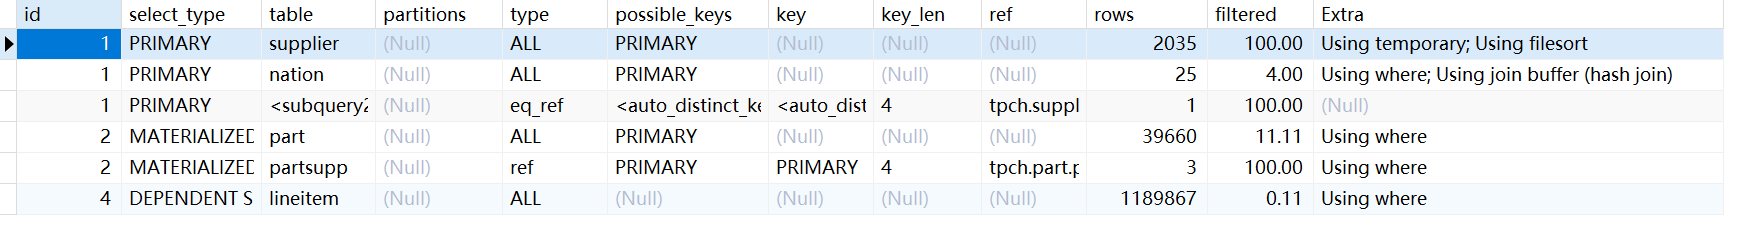
\includegraphics[width=1\textwidth]{img/39.png}
\caption{Q20查询 \tt{EXPLAIN} 结果}
\end{figure}

\begin{figure}[H]
\centering
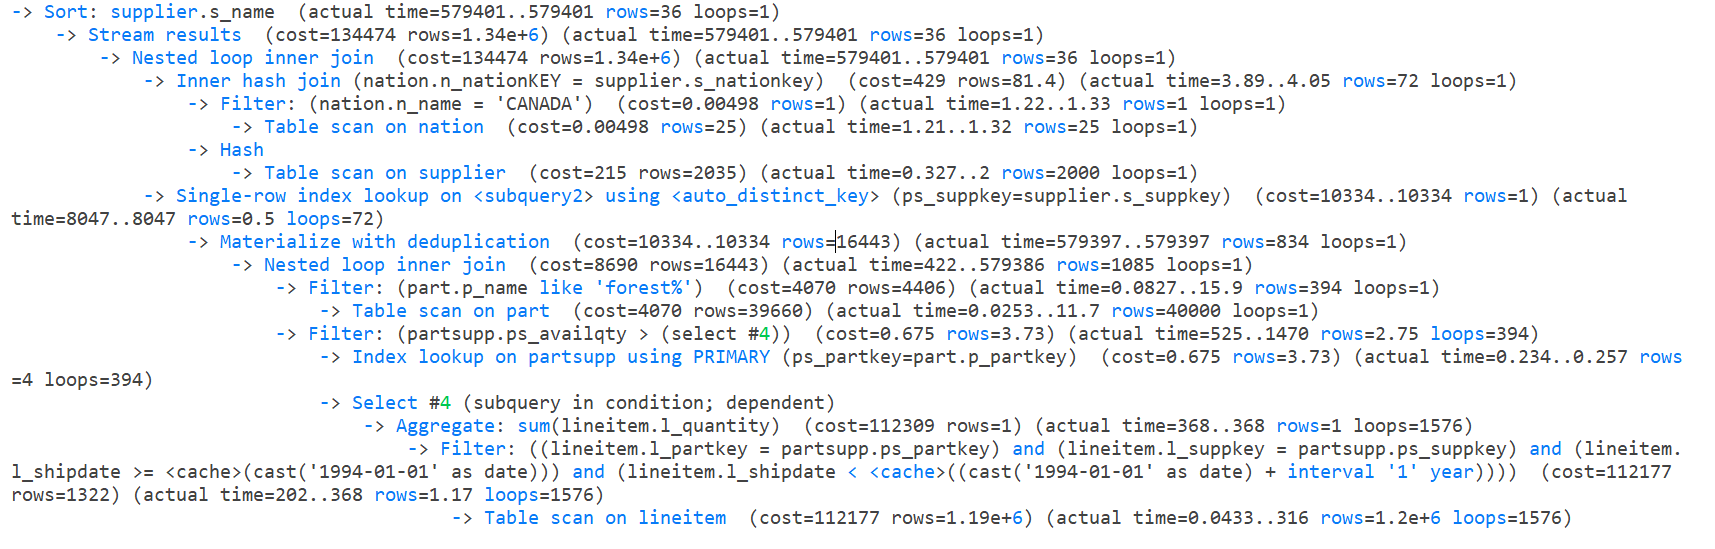
\includegraphics[width=1\textwidth]{img/40.png}
\caption{Q20查询 \tt{EXPLAIN ANALYZE} 结果}
\end{figure}


\begin{figure}[H]
  \centering
  \resizebox{\textwidth}{!}{
    \begin{forest}
    for tree={
      grow=south,
      draw,
      rounded corners,
      edge={->},
      node options={align=center, text width=15em}
    }
    [Sort: supplier.s\_name
        [Stream results
            [Nested loop inner join
                [Inner hash join (nation.n\_nationKEY \tt{=} supplier.s\_nationkey)
                    [Filter: (nation.n\_name \tt{=} 'CANADA')
                        [Table scan on nation]
                    ]
                    [Hash
                        [Table scan on supplier]
                    ]
                ]
                [Single-row index lookup on <subquery2> using <auto\_distinct\_key> (ps\_suppkey\tt{=}supplier.s\_suppkey)
                    [Materialize with deduplication
                        [Nested loop inner join
                            [Filter: (part.p\_name like 'forest\%')
                                [Table scan on part]
                            ]
                            [Filter: (partsupp.ps\_availqty > (select \#4))
                                [Index lookup on partsupp using PRIMARY (ps\_partkey\tt{=}part.p\_partkey)]
                                [Select \#4 (subquery in condition; dependent)
                                    [Aggregate: sum(lineitem.l\_quantity)
                                        [Filter
                                            [Table scan on lineitem]
                                        ]
                                    ]
                                ]
                            ]
                        ]
                    ]
                ]
            ]
        ]
    ]
    \end{forest}
  }
  \caption{Q20 查询执行计划}
\end{figure}

可以看到,Q20查询的执行计划中,对 \tt{part},\tt{nation},\tt{lineitem} 和 \tt{supplier} 表进行了全表扫描,没有使用索引,导致查询性能较差。可以通过为 \tt{part},\tt{nation},\tt{lineitem} 和 \tt{supplier} 表的相关字段创建索引来优化查询性能。

从 \tt{cost} 上看,\tt{lineitem} 表的扫描成本最高,因此应优先优化 \tt{lineitem} 表的查询性能。

\item Q21

\begin{lstlisting}[language=sql]
select s_name, count(*) as numwait 
from supplier, lineitem l1, orders, nation 
where 
  s_suppkey = l1.l_suppkey and o_orderkey = l1.l_orderkey and o_orderstatus = 'F' 
  and l1.l_receiptdate > l1.l_commitdate 
  and exists (
    select * from lineitem l2 
    where l2.l_orderkey = l1.l_orderkey 
      and l2.l_suppkey <> l1.l_suppkey 
  ) and not exists ( 
    select * from lineitem l3 
    where l3.l_orderkey = l1.l_orderkey 
      and l3.l_suppkey <> l1.l_suppkey and l3.l_receiptdate > l3.l_commitdate 
  ) and s_nationkey = n_nationkey 
  and n_name = 'SAUDI ARABIA' 
group by s_name 
order by numwait desc, s_name;
\end{lstlisting}

\begin{figure}[H]
\centering
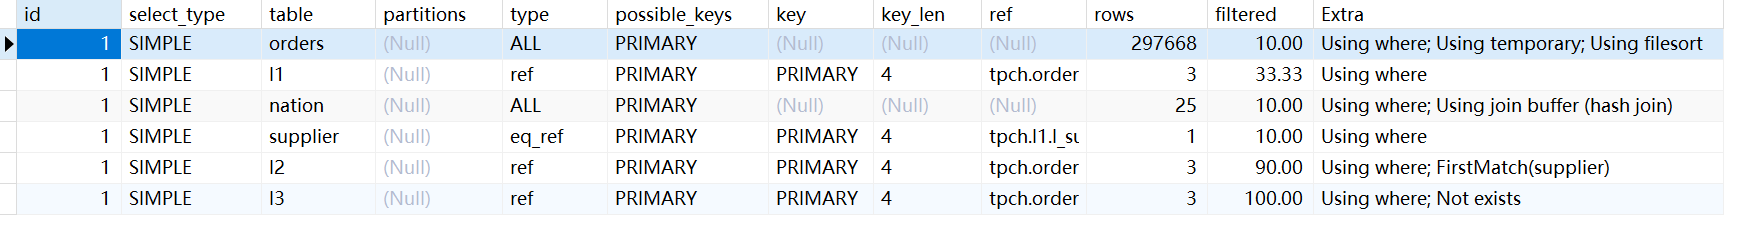
\includegraphics[width=1\textwidth]{img/41.png}
\caption{Q21查询 \tt{EXPLAIN} 结果}
\end{figure}

\begin{figure}[H]
\centering
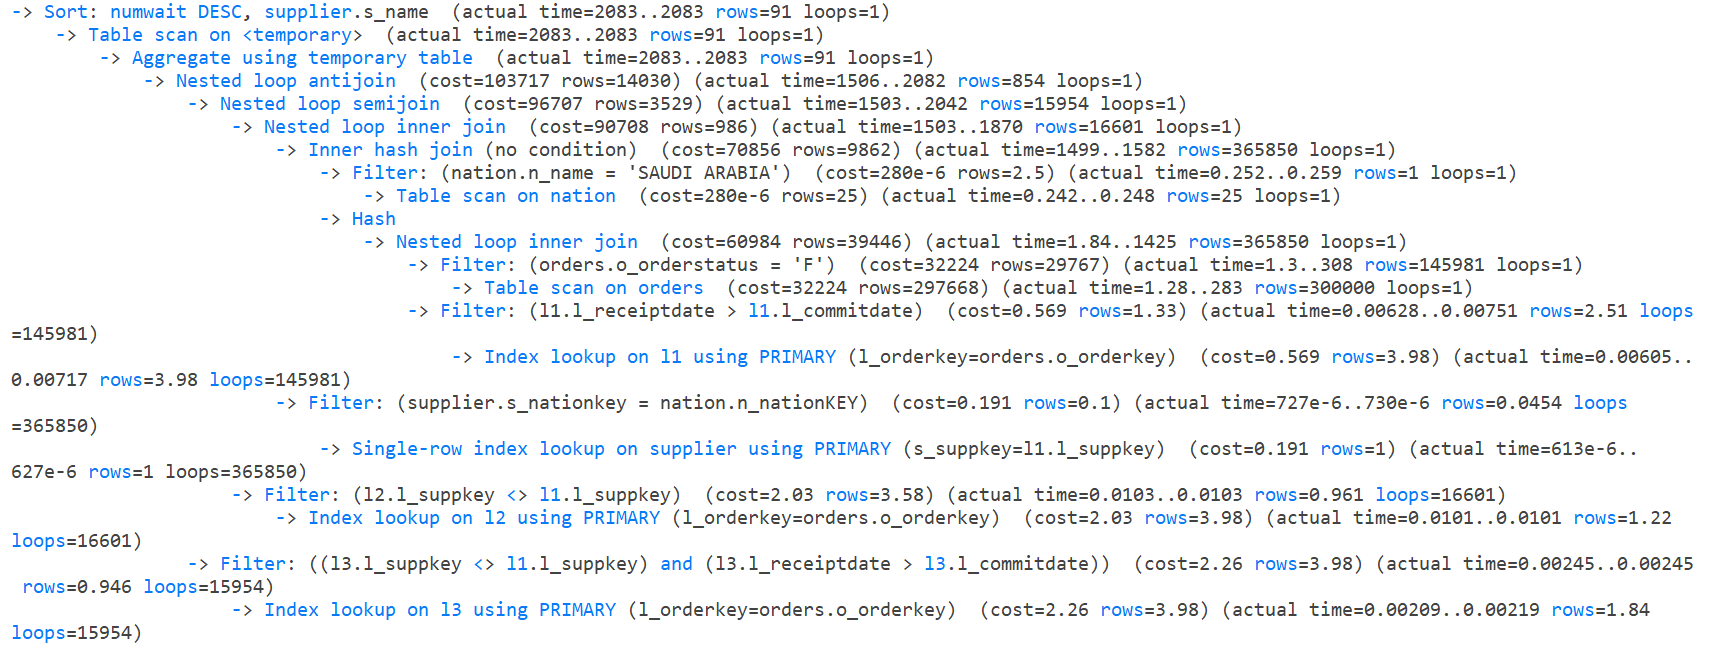
\includegraphics[width=1\textwidth]{img/42.png}
\caption{Q21查询 \tt{EXPLAIN ANALYZE} 结果}
\end{figure}

\begin{figure}[H]
  \centering
  \resizebox{\textwidth}{!}{
    \begin{forest}
    for tree={
      grow=south,
      draw,
      rounded corners,
      edge={->},
      node options={align=center, text width=10em}
    }
    [Sort: \tt{numwait DESC, supplier.s\_name}
        [Table scan on <temporary>
            [Aggregate using temporary table
                [Nested loop antijoin
                    [Nested loop semijoin
                        [Nested loop inner join
                            [Inner hash join (no condition)
                                [Filter: (nation.n\_name \tt{=} 'SAUDI ARABIA')
                                    [Table scan on nation]
                                ]
                                [Hash
                                    [Nested loop inner join
                                        [Filter: (orders.o\_orderstatus \tt{=} 'F')
                                            [Table scan on orders]
                                        ]
                                        [Filter: (l1.l\_receiptdate > l1.l\_commitdate)
                                            [Index lookup on l1 using PRIMARY (l\_orderkey \tt{=} orders.o\_orderkey)]
                                        ]
                                    ]
                                ]
                            ]
                            [Filter: (supplier.s\_nationkey \tt{=} nation.n\_nationKEY)
                                [Single-row index lookup on supplier using PRIMARY (s\_suppkey \tt{=} l1.l\_suppkey)]
                            ]
                        ]
                        [Filter: (l2.l\_suppkey <> l1.l\_suppkey)
                            [Index lookup on l2 using PRIMARY (l\_orderkey \tt{=} orders.o\_orderkey)]
                        ]
                    ]
                    [Filter: ((l3.l\_suppkey <> l1.l\_suppkey) and (l3.l\_receiptdate > l3.l\_commitdate))
                        [Index lookup on l3 using PRIMARY (l\_orderkey \tt{=} orders.o\_orderkey)]
                    ]
                ]
            ]
        ]
    ]
    \end{forest}
  }
  \caption{Q21 查询执行计划}
\end{figure}

可以看到,Q21查询的执行计划中,对 \tt{orders}和\tt{nation}  表进行了全表扫描,没有使用索引,导致查询性能较差。可以通过为 \tt{orders}和\tt{nation} 表的相关字段创建索引来优化查询性能。

从 \tt{cost} 上看,\tt{orders} 表的扫描成本最高,因此应优先优化 \tt{orders} 表的查询性能。

\item Q22

\begin{lstlisting}[language=sql]
SELECT
	cntrycode, count(*) AS numcust, sum(c_acctbal) AS totacctbal 
FROM (
	SELECT substring(c_phone FROM 1 FOR 2) AS cntrycode, c_acctbal 
	FROM customer 
	WHERE
		substring(c_phone FROM 1 FOR 2) IN ( '13', '31', '23', '29', '30', '18', '17' ) 
		AND c_acctbal > (
			SELECT avg(c_acctbal) FROM customer 
		WHERE
			c_acctbal > 0.00 
			AND substring(c_phone FROM 1 FOR 2) IN ( '13', '31', '23', '29', '30', '18', '17' ) 
		) 
		AND NOT EXISTS (SELECT * FROM orders WHERE o_custkey = c_custkey) 
) AS custsale 
GROUP BY cntrycode 
ORDER BY cntrycode;
\end{lstlisting}

\begin{figure}[H]
\centering
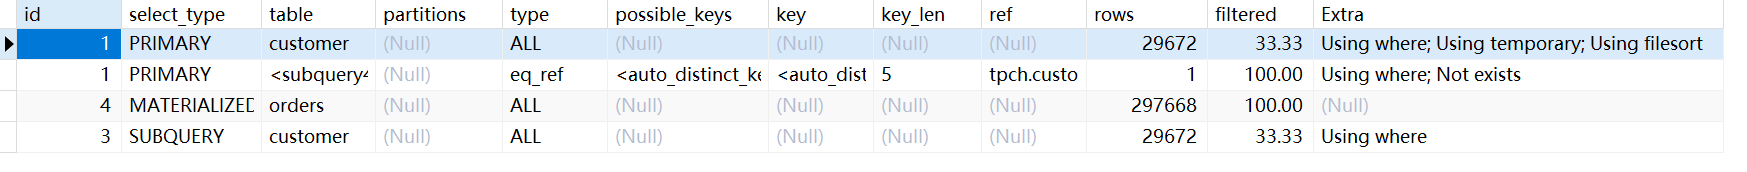
\includegraphics[width=1\textwidth]{img/43.png}
\caption{Q22查询 \tt{EXPLAIN} 结果}
\end{figure}

\begin{figure}[H]
\centering
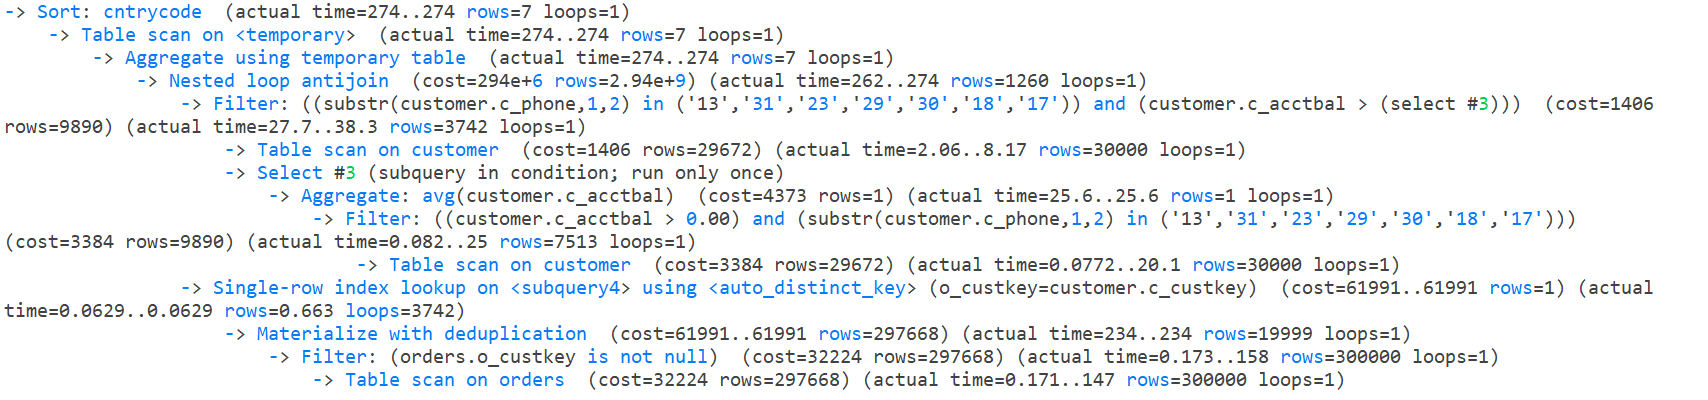
\includegraphics[width=1\textwidth]{img/44.png}
\caption{Q22查询 \tt{EXPLAIN ANALYZE} 结果}
\end{figure}

\begin{figure}[H]
  \centering
  \resizebox{\textwidth}{!}{
    \begin{forest}
    for tree={
      grow=south,
      draw,
      rounded corners,
      edge={->},
      node options={align=center, text width=15em}
    }
    [Sort: cntrycode
        [Table scan on <temporary>
            [Aggregate using temporary table
                [Nested loop antijoin
                    [Filter
                        [Table scan on customer]
                        [Select \#3 (subquery in condition; run only once)
                            [Aggregate: avg(customer.c\_acctbal)
                                [Filter
                                    [Table scan on customer]
                                ]
                            ]
                        ]
                    ]
                    [Single-row index lookup on <subquery4> using <auto\_distinct\_key> (o\_custkey \tt{=} customer.c\_custkey)
                        [Materialize with deduplication
                            [Filter: (orders.o\_custkey is not null)
                                [Table scan on orders]
                            ]
                        ]
                    ]
                ]
            ]
        ]
    ]
    \end{forest}
  }
  \caption{Q22 查询执行计划}
\end{figure}

可以看到,Q22查询的执行计划中,对 \tt{customer}和\tt{orders} 表进行了全表扫描,没有使用索引,导致查询性能较差。可以通过为 \tt{customer}和\tt{orders} 表的相关字段创建索引来优化查询性能。

从 \tt{cost} 上看,\tt{orders} 表的扫描成本最高,因此应优先优化 \tt{orders} 表的查询性能。

\end{enumerate}

\subsubsection{优化}

根据上述分析,我们可以为相关表的相关字段创建索引来优化查询性能。建立索引后,再次使用 \tt{EXPLAIN} 和 \tt{EXPLAIN ANALYZE} 查看查询执行计划,分析优化效果。

\begin{enumerate}
  \item Q1

为 \tt{lineitem} 表的 \tt{l\_shipdate} 字段创建索引。

\begin{figure}[H]
\centering
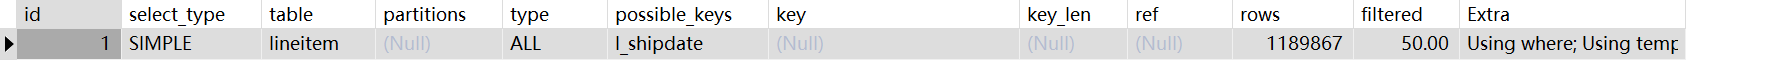
\includegraphics[width=0.9\textwidth]{img/45.png}
\caption{Q1查询优化后 \tt{EXPLAIN} 结果}
\end{figure}

\begin{figure}[H]
\centering
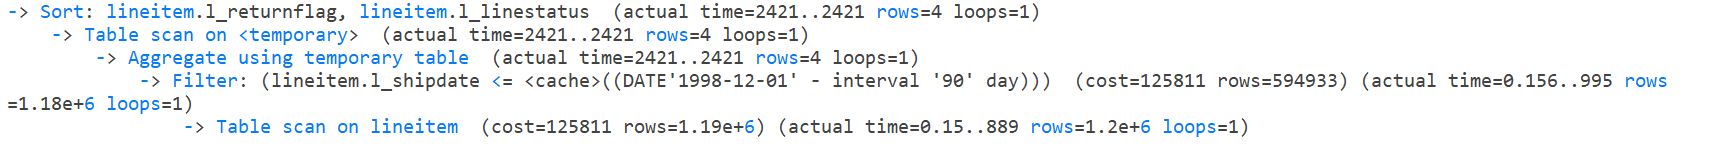
\includegraphics[width=0.9\textwidth]{img/46.png}
\caption{Q1查询优化后 \tt{EXPLAIN ANALYZE} 结果}
\end{figure}

可以发现,由于 Q1 查询中聚合函数较多,因此优化效果不明显。

  \item Q2
  
为 \tt{part} 表的 \tt{p\_partkey}, \tt{p\_size}和\tt{p\_type} 字段,\tt{region} 表的\tt{r\_regionkey}和\tt{r\_name}字段创建索引。

\begin{figure}[H]
\centering
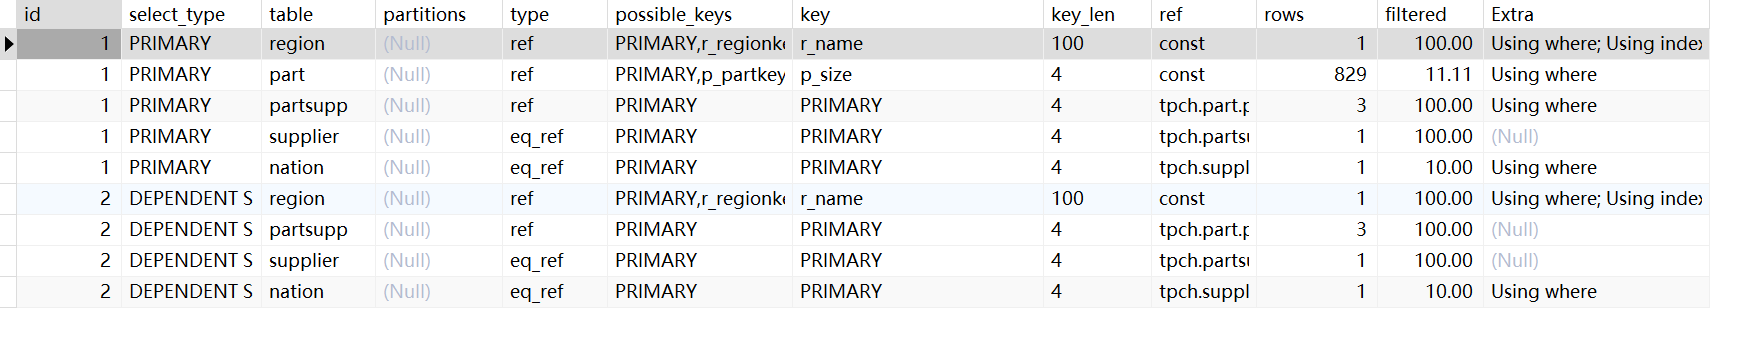
\includegraphics[width=0.9\textwidth]{img/47.png}
\caption{Q2查询优化后 \tt{EXPLAIN} 结果}
\end{figure}

\begin{figure}[H]
\centering
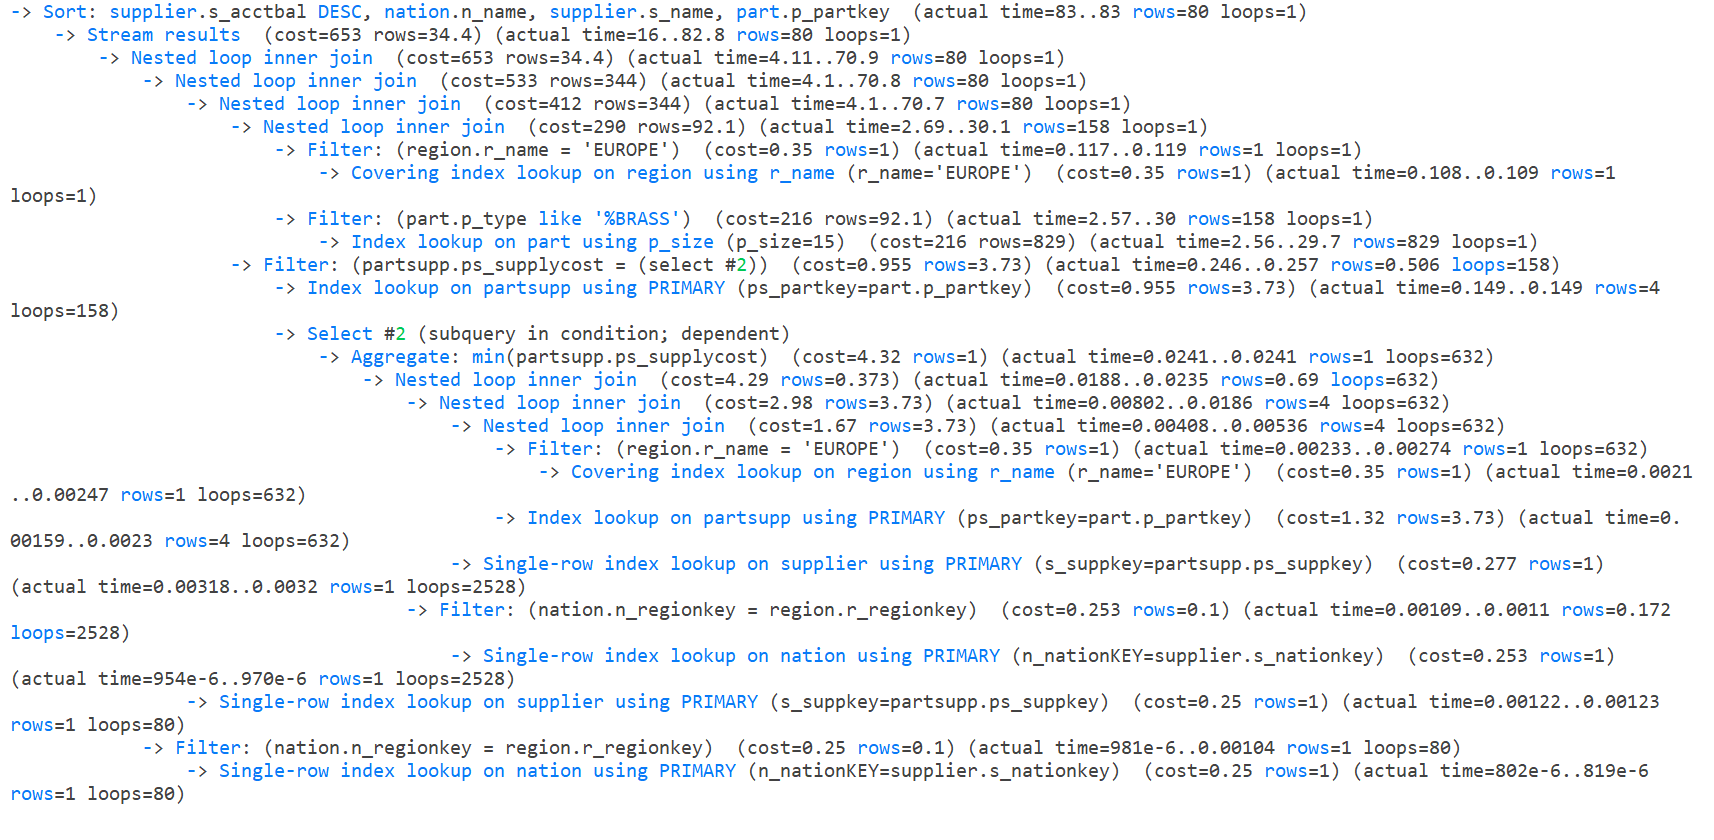
\includegraphics[width=0.9\textwidth]{img/48.png}
\caption{Q2查询优化后 \tt{EXPLAIN ANALYZE} 结果}
\end{figure}

可以发现,Q2查询的新执行计划中,避免了全表扫描,且 \tt{cost} 明显降低,优化效果明显。

  \item Q3
  
为 \tt{orders} 表的 \tt{o\_orderdate} 字段创建索引。

\begin{figure}[H]
\centering
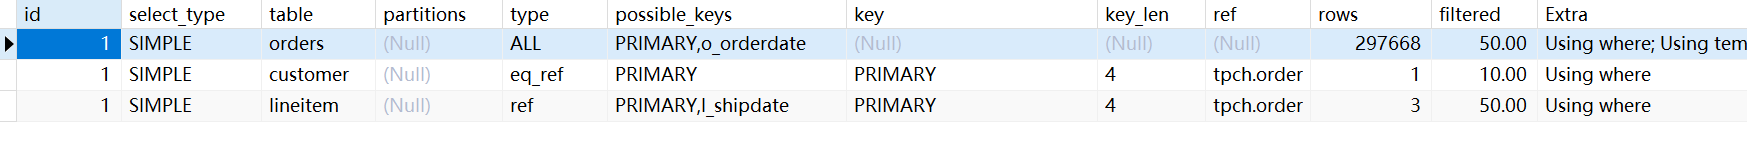
\includegraphics[width=0.9\textwidth]{img/49.png}
\caption{Q3查询优化后 \tt{EXPLAIN} 结果}
\end{figure}

\begin{figure}[H]
\centering
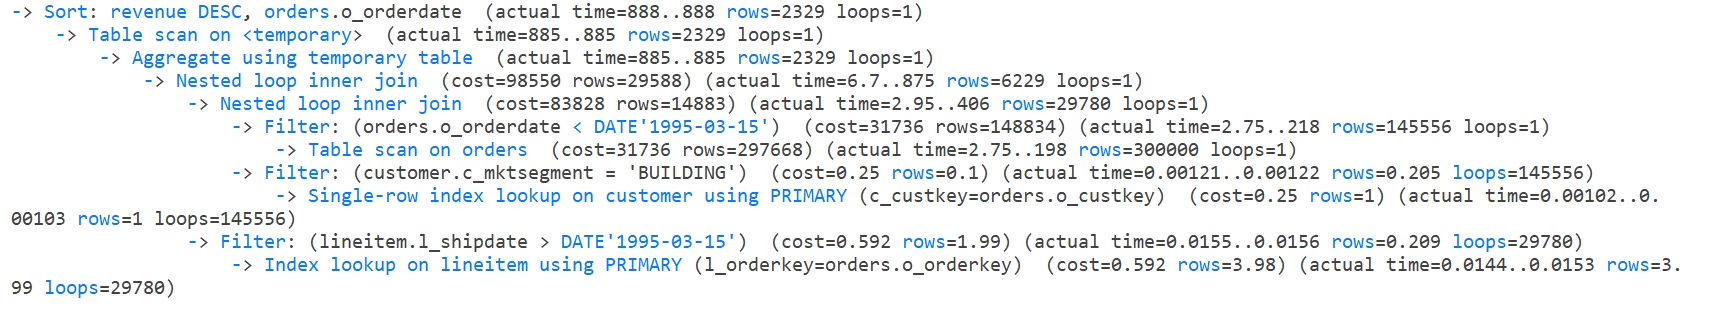
\includegraphics[width=0.9\textwidth]{img/50.png}
\caption{Q3查询优化后 \tt{EXPLAIN ANALYZE} 结果}
\end{figure}

优化效果不明显,未能避免全表扫描。

  \item Q4
  
先前已对 \tt{orders} 表的 \tt{o\_orderdate} 字段创建索引,因此无需再次优化。

\begin{figure}[H]
\centering
\includegraphics[width=0.9\textwidth]{img/51.png}
\caption{Q4查询优化后 \tt{EXPLAIN} 结果}
\end{figure}

\begin{figure}[H]
\centering
\includegraphics[width=0.9\textwidth]{img/52.png}
\caption{Q4查询优化后 \tt{EXPLAIN ANALYZE} 结果}
\end{figure}

可以发现,Q4查询的新执行计划中,避免了全表扫描,且 \tt{cost} 明显降低,优化效果明显。

  \item Q5
  
为 \tt{orders},\tt{nation}和 \tt{customer} 表的相关字段创建索引。

\begin{figure}[H]
\centering
\includegraphics[width=0.9\textwidth]{img/53.png}
\caption{Q5查询优化后 \tt{EXPLAIN} 结果}
\end{figure}

\begin{figure}[H]
\centering
\includegraphics[width=0.9\textwidth]{img/54.png}
\caption{Q5查询优化后 \tt{EXPLAIN ANALYZE} 结果}
\end{figure}

可以发现,Q5查询的新执行计划中,避免了一些表的全表扫描,且 \tt{cost} 降低,有优化效果。

  \item Q6
  
通过添加索引未能继续优化查询性能。

\begin{figure}[H]
\centering
\includegraphics[width=0.9\textwidth]{img/55.png}
\caption{Q6查询优化后 \tt{EXPLAIN} 结果}
\end{figure}

\begin{figure}[H]
\centering
\includegraphics[width=0.9\textwidth]{img/56.png}
\caption{Q6查询优化后 \tt{EXPLAIN ANALYZE} 结果}
\end{figure}

  \item Q7
  
在优化其他查询时,已为相关表的相关字段创建索引,因此无需继续优化。

\begin{figure}[H]
\centering
\includegraphics[width=0.9\textwidth]{img/57.png}
\caption{Q7查询优化后 \tt{EXPLAIN} 结果}
\end{figure}

\begin{figure}[H]
\centering
\includegraphics[width=0.9\textwidth]{img/58.png}
\caption{Q7查询优化后 \tt{EXPLAIN ANALYZE} 结果}
\end{figure}

可以发现,Q7查询的新执行计划中,避免了一些表的全表扫描,且 \tt{cost} 降低,有优化效果。

  \item Q8
  
在优化其他查询时,已为相关表的相关字段创建索引,因此无需继续优化。

\begin{figure}[H]
\centering
\includegraphics[width=0.9\textwidth]{img/59.png}
\caption{Q8查询优化后 \tt{EXPLAIN} 结果}
\end{figure}

\begin{figure}[H]
\centering
\includegraphics[width=0.9\textwidth]{img/60.png}
\caption{Q8查询优化后 \tt{EXPLAIN ANALYZE} 结果}
\end{figure}

可以发现,Q8查询的新执行计划中,避免了一些表的全表扫描,且 \tt{cost} 降低,有优化效果。

  \item Q9
  
为 \tt{lineitem} 表和\tt{part} 表的相关字段创建索引。

\begin{figure}[H]
\centering
\includegraphics[width=0.9\textwidth]{img/61.png}
\caption{Q9查询优化后 \tt{EXPLAIN} 结果}
\end{figure}

\begin{figure}[H]
\centering
\includegraphics[width=0.9\textwidth]{img/62.png}
\caption{Q9查询优化后 \tt{EXPLAIN ANALYZE} 结果}
\end{figure}

可以发现,Q9查询的新执行计划中,避免了一些表的全表扫描,且 \tt{cost} 降低,有优化效果。

  \item Q10
  
为相关表的相关字段创建索引。

\begin{figure}[H]
\centering
\includegraphics[width=0.9\textwidth]{img/63.png}
\caption{Q10查询优化后 \tt{EXPLAIN} 结果}
\end{figure}

\begin{figure}[H]
\centering
\includegraphics[width=0.9\textwidth]{img/64.png}
\caption{Q10查询优化后 \tt{EXPLAIN ANALYZE} 结果}
\end{figure}

可以发现,Q10查询的新执行计划中,避免了一些表的全表扫描,且 \tt{cost} 降低,有优化效果。

  \item Q11
  
创建索引后,未能避免全表扫描。

\begin{figure}[H]
\centering
\includegraphics[width=0.9\textwidth]{img/65.png}
\caption{Q11查询优化后 \tt{EXPLAIN} 结果}
\end{figure}

\begin{figure}[H]
\centering
\includegraphics[width=0.9\textwidth]{img/66.png}
\caption{Q11查询优化后 \tt{EXPLAIN ANALYZE} 结果}
\end{figure}

优化效果不明显。

  \item Q12
  
创建索引后,未能避免全表扫描。

\begin{figure}[H]
\centering
\includegraphics[width=0.9\textwidth]{img/67.png}
\caption{Q12查询优化后 \tt{EXPLAIN} 结果}
\end{figure}

\begin{figure}[H]
\centering
\includegraphics[width=0.9\textwidth]{img/68.png}
\caption{Q12查询优化后 \tt{EXPLAIN ANALYZE} 结果}
\end{figure}

优化效果不明显。

  \item Q13
  
在优化其他查询时,已为相关表的相关字段创建索引,因此无需继续优化。

\begin{figure}[H]
\centering
\includegraphics[width=0.9\textwidth]{img/69.png}
\caption{Q13查询优化后 \tt{EXPLAIN} 结果}
\end{figure}

\begin{figure}[H]
\centering
\includegraphics[width=0.9\textwidth]{img/70.png}
\caption{Q13查询优化后 \tt{EXPLAIN ANALYZE} 结果}
\end{figure}

可以发现,Q13查询的新执行计划中,避免了\tt{customer} 表的全表扫描,且 \tt{cost} 降低,有优化效果。

  \item Q14
  
在优化其他查询时,已为相关表的相关字段创建索引,因此无需继续优化。

\begin{figure}[H]
\centering
\includegraphics[width=0.9\textwidth]{img/71.png}
\caption{Q14查询优化后 \tt{EXPLAIN} 结果}
\end{figure}

\begin{figure}[H]
\centering
\includegraphics[width=0.9\textwidth]{img/72.png}
\caption{Q14查询优化后 \tt{EXPLAIN ANALYZE} 结果}
\end{figure}

可以发现,Q14查询的新执行计划中,避免了\tt{lineitem} 表的全表扫描,且 \tt{cost} 降低,有优化效果。

  \item Q15
  
在优化其他查询时,已为相关表的相关字段创建索引,因此无需继续优化。

\begin{figure}[H]
\centering
\includegraphics[width=0.9\textwidth]{img/73.png}
\caption{Q15查询优化后 \tt{EXPLAIN} 结果}
\end{figure}

\begin{figure}[H]
\centering
\includegraphics[width=0.9\textwidth]{img/74.png}
\caption{Q15查询优化后 \tt{EXPLAIN ANALYZE} 结果}
\end{figure}

可以发现,Q15查询的新执行计划中,避免了\tt{lineitem} 表的全表扫描,且 \tt{cost} 降低,有优化效果。

  \item Q16
  
为 \tt{part}和\tt{supplier} 表的相关字段创建索引。

\begin{figure}[H]
\centering
\includegraphics[width=0.9\textwidth]{img/75.png}
\caption{Q16查询优化后 \tt{EXPLAIN} 结果}
\end{figure}

\begin{figure}[H]
\centering
\includegraphics[width=0.9\textwidth]{img/76.png}
\caption{Q16查询优化后 \tt{EXPLAIN ANALYZE} 结果}
\end{figure}

可以发现,Q16查询的新执行计划中,避免了\tt{part}和\tt{supplier} 表的全表扫描,且 \tt{cost} 降低,有优化效果。

  \item Q17
  
先前已对 \tt{lineitem} 表和\tt{part}表创建索引,因此无需再次优化。

\begin{figure}[H]
\centering
\includegraphics[width=0.9\textwidth]{img/77.png}
\caption{Q17查询优化后 \tt{EXPLAIN} 结果}
\end{figure}

\begin{figure}[H]
\centering
\includegraphics[width=0.9\textwidth]{img/78.png}
\caption{Q17查询优化后 \tt{EXPLAIN ANALYZE} 结果}
\end{figure}

可以发现,Q17查询的新执行计划中,避免了\tt{lineitem}和\tt{part} 表的全表扫描,且 \tt{cost} 明显降低,优化效果显著。

  \item Q18
  
创建索引后,未能避免全表扫描。

\begin{figure}[H]
\centering
\includegraphics[width=0.9\textwidth]{img/79.png}
\caption{Q18查询优化后 \tt{EXPLAIN} 结果}
\end{figure}

\begin{figure}[H]
\centering
\includegraphics[width=0.9\textwidth]{img/80.png}
\caption{Q18查询优化后 \tt{EXPLAIN ANALYZE} 结果}
\end{figure}

优化效果不明显。

  \item Q19
  
在优化其他查询时,已为相关表的相关字段创建索引,因此无需继续优化。

\begin{figure}[H]
\centering
\includegraphics[width=0.9\textwidth]{img/81.png}
\caption{Q19查询优化后 \tt{EXPLAIN} 结果}
\end{figure}

\begin{figure}[H]
\centering
\includegraphics[width=0.9\textwidth]{img/82.png}
\caption{Q19查询优化后 \tt{EXPLAIN ANALYZE} 结果}
\end{figure}

可以发现,Q19查询的新执行计划中,避免了\tt{part} 表的全表扫描,且 \tt{cost} 降低,有优化效果。

  \item Q20
  
在优化其他查询时,已为相关表的相关字段创建索引,因此无需继续优化。

\begin{figure}[H]
\centering
\includegraphics[width=0.9\textwidth]{img/83.png}
\caption{Q20查询优化后 \tt{EXPLAIN} 结果}
\end{figure}

\begin{figure}[H]
\centering
\includegraphics[width=0.9\textwidth]{img/84.png}
\caption{Q20查询优化后 \tt{EXPLAIN ANALYZE} 结果}
\end{figure}

可以发现,Q20查询的新执行计划中,避免了\tt{part},\tt{supplier},\tt{nation},\tt{lineitem} 表的全表扫描,且 \tt{cost} 明显降低,优化效果显著。

  \item Q21
  
为 \tt{orders} 表的 \tt{o\_orderstatus} 字段创建索引。

\begin{figure}[H]
\centering
\includegraphics[width=0.9\textwidth]{img/85.png}
\caption{Q21查询优化后 \tt{EXPLAIN} 结果}
\end{figure}

\begin{figure}[H]
\centering
\includegraphics[width=0.9\textwidth]{img/86.png}
\caption{Q21查询优化后 \tt{EXPLAIN ANALYZE} 结果}
\end{figure}

可以发现,Q21查询的新执行计划中,避免了\tt{orders} 表的全表扫描,且 \tt{cost} 降低,有优化效果。

  \item Q22
  
创建索引后,未能避免全表扫描。

\begin{figure}[H]
\centering
\includegraphics[width=0.9\textwidth]{img/87.png}
\caption{Q22查询优化后 \tt{EXPLAIN} 结果}
\end{figure}

\begin{figure}[H]
\centering
\includegraphics[width=0.9\textwidth]{img/88.png}
\caption{Q22查询优化后 \tt{EXPLAIN ANALYZE} 结果}
\end{figure}

优化效果不明显。


\end{enumerate}

\subsubsection{课程项目查询分析}

\begin{itemize}
  \item 创建课程项目所使用的数据库环境,并导入全量的数据集;
  \item 针对课程项目 任务5 中所设计查询,使用 \tt{EXPLAIN} 进行分析;
  \begin{itemize}[label=\(\circ\)]
    \item 画出查询计划树,并说明每个节点的功能和执行时间等信息;
    \item 说明该执行计划是否是最优的;
    \item 针对可能存在的性能问题,提出解决方案;
  \end{itemize}
\end{itemize}

我们选取了部分查询进行分析,如下:

\begin{enumerate}
  \item Q1
  \begin{lstlisting}[language=sql]
SELECT * FROM "user" WHERE email = 'test_email';
\end{lstlisting}

\begin{figure}[H]
\centering
\includegraphics[width=0.9\textwidth]{img/89.png}
\caption{Q1 查询 \tt{EXPLAIN ANALYZE} 结果}
\end{figure}

\begin{figure}[H]
  \centering
  % \resizebox{\textwidth}{!}{
    \begin{forest}
    for tree={
      grow=south,
      draw,
      rounded corners,
      edge={->},
      node options={align=center, text width=10em}
    }
    [Seq Scan on \tt{"user"}
      [Filter: (\tt{(email)::text = 'test\_email'::text})]
    ]
    \end{forest}
  % }
  \caption{Q1查询执行计划}
\end{figure}

是最优的计划。

\item Q2

\begin{lstlisting}[language=sql]
SELECT * FROM "history" WHERE user_id = 0;
\end{lstlisting}

\begin{figure}[H]
\centering
\includegraphics[width=0.9\textwidth]{img/90.png}
\caption{Q2查询 \tt{EXPLAIN ANALYZE} 结果}
\end{figure}

\begin{figure}[H]
  \centering
  % \resizebox{\textwidth}{!}{
    \begin{forest}
    for tree={
      grow=south,
      draw,
      rounded corners,
      edge={->},
      node options={align=center, text width=10em}
    }
    [Seq Scan on \tt{history}
      [Filter: \tt{(user\_id = 0)}]
    ]
    \end{forest}
  % }
  \caption{Q2查询执行计划}
\end{figure}

是最优的计划。

\item Q3

\begin{lstlisting}[language=sql]
SELECT * FROM author WHERE name LIKE '%' || 'aa' || '%';
\end{lstlisting}

\begin{figure}[H]
\centering
\includegraphics[width=0.9\textwidth]{img/91.png}
\caption{Q3查询 \tt{EXPLAIN ANALYZE} 结果}
\end{figure}

\begin{figure}[H]
  \centering
  % \resizebox{\textwidth}{!}{
    \begin{forest}
    for tree={
      grow=south,
      draw,
      rounded corners,
      edge={->},
      node options={align=center, text width=10em}
    }
    [Gather
      [Parallel Seq Scan on \tt{author}
        [Filter: \tt{(name)::text \textasciitilde \textasciitilde '\%aa\%'::text}]
      ]
    ]
    \end{forest}
  % }
  \caption{Q3查询执行计划}
\end{figure}

是最优的计划。但可以考虑使用插件优化模糊搜索。

\item Q4

\begin{lstlisting}[language=sql]
SELECT w.author_name, ar.id, ar.title, ar.abstract, ar.doi, ar.license, ar.publish_time, ar.url
FROM "write" w
JOIN article ar ON w.article_id = ar.id
WHERE w.author_name LIKE '%' || 'aa' || '%';
\end{lstlisting}

\begin{figure}[H]
\centering
\includegraphics[width=0.9\textwidth]{img/92.png}
\caption{Q4查询 \tt{EXPLAIN ANALYZE} 结果}
\end{figure}

\begin{figure}[H]
  \centering
  % \resizebox{\textwidth}{!}{
    \begin{forest}
    for tree={
      grow=south,
      draw,
      rounded corners,
      edge={->},
      node options={align=center, text width=10em}
    }
    [Gather
      [Nested Loop
        [Parallel Seq Scan on \tt{write w}
          [Filter: \tt{(author\_name)::text \textasciitilde \textasciitilde '\%aa\%'::text}]
        ]
        [Index Scan using \tt{idx\_article\_id} on \tt{article ar}
          [Index Cond: \tt{(id)::text = (w.article\_id)::text}]
        ]
      ]
    ]
    \end{forest}
  % }
  \caption{Q4查询执行计划}
\end{figure}

由于使用了索引,是最优的计划。但可以考虑使用插件优化模糊搜索。

\item Q5

\begin{lstlisting}[language=sql]
SELECT ar.id, ar.title, ar.abstract, ar.doi, ar.license
FROM article ar
JOIN publish p ON ar.id = p.article_id
JOIN "write" w ON ar.id = w.article_id
WHERE ar.title LIKE '%' || 'aa' || '%';
\end{lstlisting}

\begin{figure}[H]
\centering
\includegraphics[width=0.9\textwidth]{img/93.png}
\caption{Q5查询 \tt{EXPLAIN ANALYZE} 结果}
\end{figure}

\begin{figure}[H]
  \centering
  \resizebox{\textwidth}{!}{
    \begin{forest}
    for tree={
      grow=south,
      draw,
      rounded corners,
      edge={->},
      node options={align=center, text width=10em}
    }
    [Gather
      [Nested Loop
        [Join Filter: \tt{(ar.id)::text = (w.article\_id)::text}]
        [Nested Loop
          [Parallel Seq Scan on \tt{article ar}
            [Filter: \tt{(title \textasciitilde\textasciitilde '\%aa\%'::text)}]
          ]
          [Index Only Scan using \tt{idx\_publish\_arid} on \tt{publish p}
            [Index Cond: \tt{(article\_id = (ar.id)::text)}]
            [Heap Fetches: 3]
          ]
        ]
        [Index Only Scan using \tt{idx\_write\_aeid} on \tt{write w}
          [Index Cond: \tt{(article\_id = (p.article\_id)::text)}]
          [Heap Fetches: 0]
        ]
      ]
    ]
    \end{forest}
  }
  \caption{Q5查询执行计划}
\end{figure}

由于使用了索引,是最优的计划。但可以考虑使用插件优化模糊搜索。

\item Q6

\begin{lstlisting}[language=sql]
SELECT ar.id, w.author_name, ar.title, ar.abstract, ar.doi, ar.license, 
  ar.publish_time, ar.url, p.journal_name
FROM article ar
JOIN publish p ON ar.id = p.article_id
JOIN write w ON ar.id = w.article_id
WHERE ar.study_type LIKE '%' || 'testst' || '%'
  OR ar.addressed_population LIKE '%' || 'testadd' || '%'
  OR ar.challenge LIKE '%' || 'testcl' || '%'
  OR ar.focus LIKE '%' || 'testfo' || '%';
\end{lstlisting}

\begin{figure}[H]
\centering
\includegraphics[width=0.9\textwidth]{img/94.png}
\caption{Q6查询 \tt{EXPLAIN ANALYZE} 结果}
\end{figure}

\begin{figure}[H]
  \centering
  \resizebox{\textwidth}{!}{
    \begin{forest}
    for tree={
      grow=south,
      draw,
      rounded corners,
      edge={->},
      node options={align=center, text width=10em}
    }
    [Nested Loop
      [Join Filter: \tt{(ar.id)::text = (w.article\_id)::text}]
      [Nested Loop
        [Gather
          [Parallel Seq Scan on \tt{article ar}
            [Filter: \tt{((study\_type)::text \textasciitilde\textasciitilde '\%testst\%'::text) OR ((addressed\_population)::text \textasciitilde\textasciitilde '\%testadd\%'::text) OR ((challenge)::text \textasciitilde\textasciitilde '\%testcl\%'::text) OR ((focus)::text \textasciitilde\textasciitilde '\%testfo\%'::text)}]
          ]
        ]
        [Index Scan using \tt{idx\_publish\_arid} on \tt{publish p}
          [Index Cond: \tt{(article\_id)::text = (ar.id)::text}]
        ]
      ]
      [Index Scan using \tt{idx\_write\_aeid} on \tt{write w}
        [Index Cond: \tt{(article\_id)::text = (p.article\_id)::text}]
      ]
    ]
    \end{forest}
  }
  \caption{Q6查询执行计划}

由于使用了索引,是最优的计划。但可以考虑使用插件优化模糊搜索。
\end{figure}

\item Q7

\begin{lstlisting}[language=sql]
WITH RECURSIVE c AS (
  SELECT citing_id, cited_id, 0 AS flag
  FROM cite
  UNION ALL
  SELECT cite.citing_id, cite.cited_id, 1 AS flag
  FROM c
  JOIN cite ON c.cited_id = cite.citing_id
)
SELECT * FROM c;
\end{lstlisting}

\begin{figure}[H]
\centering
\includegraphics[width=0.9\textwidth]{img/95.png}
\caption{Q7查询 \tt{EXPLAIN ANALYZE} 结果}
\end{figure}

\begin{figure}[H]
  \centering
  \resizebox{\textwidth}{!}{
    \begin{forest}
    for tree={
      grow=south,
      draw,
      rounded corners,
      edge={->},
      node options={align=center, text width=10em}
    }
    [CTE Scan on \tt{c}
      [CTE \tt{c}
        [Recursive Union
          [Seq Scan on \tt{cite}]
          [Merge Join
            [Merge Cond: \tt{(cite\_1.citing\_id)::text = (c\_1.cited\_id)::text}]
            [Index Only Scan using \tt{cite\_citing\_id\_cited\_id\_idx} on \tt{cite cite\_1}
              [Heap Fetches: 0]
            ]
            [Materialize
              [Sort Key: \tt{c\_1.cited\_id}]
              [Sort Method: external merge  Disk: 104064kB]
              [WorkTable Scan on \tt{c c\_1}]
            ]
          ]
        ]
      ]
    ]
    \end{forest}
  }
  \caption{Q7 查询执行计划}
\end{figure}

在递归查询的情况下,是比较好的计划。

\end{enumerate}



\section{存在的问题及解决方案}

\begin{enumerate}
  \item 不会分析 \tt{EXPLAIN} 和 \tt{EXPLAIN ANALYZE} 的结果。
  
  解决方案:查询网络资料,学习如何分析 \tt{EXPLAIN} 和 \tt{EXPLAIN ANALYZE} 的结果,了解如何根据执行计划优化查询性能。

  \item PostgreSQL 查询计划结果与 MySQL 格式不同。
  
  解决方案:查询 PostgreSQL 官方文档,了解 PostgreSQL 查询计划的格式,学习如何分析 PostgreSQL 查询计划。
\end{enumerate}


\section{实验小结}

通过本次实验,我学会了如何使用 \tt{EXPLAIN} 和 \tt{EXPLAIN ANALYZE} 分析查询执行计划,了解了查询执行计划的相关信息,学会了如何根据执行计划优化查询性能。同时,我也使用了 \tt{EXPLAIN} 和 \tt{EXPLAIN ANALYZE} 分析课程项目中的查询,了解了课程项目中的查询执行计划。通过本次实验,我对查询执行计划有了更深入的了解,对如何优化查询性能有了更多的认识。


\end{document}